%\documentclass[runningheads,a4paper]{lincs}
%\documentclass[sttt]{svjour}
\documentclass{template/openetcs_article}


\usepackage{xspace}
\usepackage{rotating,url,color}
\setcounter{tocdepth}{3}
\usepackage{graphicx}
\usepackage{multirow}
\usepackage[table]{xcolor}
\usepackage{datetime}
\usepackage{moreverb}
\usepackage{fancyvrb}

\urldef{\mailboth}\path|{huang,jp}@informatik.uni-bremen.de|
\newcommand{\keywords}[1]{\par\addvspace\baselineskip
\noindent {\bf Keywords} \enspace\ignorespaces#1}


\DeclareMathSymbol{\B}{\mathalpha}{AMSb}{"42}
\DeclareMathSymbol{\I}{\mathalpha}{AMSb}{"49}
\DeclareMathSymbol{\N}{\mathalpha}{AMSb}{"4E}
\DeclareMathSymbol{\Pwr}{\mathalpha}{AMSb}{"50}
\DeclareMathSymbol{\Q}{\mathalpha}{AMSb}{"51}
\DeclareMathSymbol{\R}{\mathalpha}{AMSb}{"52}
\DeclareMathSymbol{\Z}{\mathalpha}{AMSb}{"5A}
\DeclareMathSymbol{\Sol}{\mathalpha}{AMSb}{"53}

\newcommand{\ebcmd}{\mathsf{EmergencyBrakeCommand}}
\newcommand{\sbcmd}{\mathsf{ServiceBrakeCommand}}

\newcommand{\numreq}{11}
\newcommand{\numsubreq}{29}
\newcommand{\numtc}{34}

\DeclareMathSymbol{\B}{\mathalpha}{AMSb}{"42}
\DeclareMathSymbol{\I}{\mathalpha}{AMSb}{"49}
\DeclareMathSymbol{\N}{\mathalpha}{AMSb}{"4E}
\DeclareMathSymbol{\Pwr}{\mathalpha}{AMSb}{"50}
\DeclareMathSymbol{\Q}{\mathalpha}{AMSb}{"51}
\DeclareMathSymbol{\R}{\mathalpha}{AMSb}{"52}
\DeclareMathSymbol{\Z}{\mathalpha}{AMSb}{"5A}
\DeclareMathSymbol{\Sol}{\mathalpha}{AMSb}{"53}

\newcommand{\obsv}[1]{{\cal O}(#1)}
\newcommand{\ctrl}[1]{{\cal C}(#1)}
\newcommand{\vdot}[1]{\stackrel{.}{#1}}
\newcommand{\power}{\mathbf{P}}

\newcommand{\HS}{{\mathcal H}}

\newcommand{\Interval}{\I}

\newcommand{\ist}{\mbox{{\tt true}}}
\newcommand{\isf}{\mbox{{\tt false}}}
\newcommand{\emptytrace}{\langle~\rangle}
\newcommand{\abegin}{\mathbf{begin}}
\newcommand{\aend}{\mathbf{end}}
\newcommand{\alet}{\mathbf{let}}
\newcommand{\aendlet}{\mathbf{endlet}}
\newcommand{\ain}{\mathbf{in}}
\newcommand{\afor}{\mathbf{for}}
\newcommand{\adownto}{\mathbf{downto}}
\newcommand{\aforall}{\mathbf{foreach}}
\newcommand{\awhile}{\mathbf{while}}
\newcommand{\ado}{\mathbf{do}}
\newcommand{\aenddo}{\mathbf{enddo}}
\newcommand{\acontinue}{\mathbf{continue}}
\newcommand{\aif}{\mathbf{if}}
\newcommand{\athen}{\mathbf{then}}
\newcommand{\aelse}{\mathbf{else}}
\newcommand{\aelseif}{\mathbf{elseif}}
\newcommand{\aendif}{\mathbf{endif}}
\newcommand{\ainout}{\mathbf{inout}}
\newcommand{\aout}{\mathbf{out}}
\newcommand{\aprocedure}{\mathbf{procedure}}
\newcommand{\afunction}{\mathbf{function}}
\newcommand{\abreak}{\mathbf{break}}
\newcommand{\awhere}{\mathbf{where}}
\newcommand{\Sup}[1]{\overline{#1}}
\newcommand{\Inf}[1]{\underline{#1}}

\newcommand{\trl}{/\!/}



\newcommand{\taba}{\hspace*{3mm}{}}
\newcommand{\tabb}{\hspace*{6mm}{}}
\newcommand{\tabc}{\hspace*{9mm}{}}
\newcommand{\tabd}{\hspace*{12mm}{}}
\newcommand{\tabe}{\hspace*{15mm}{}}
\newcommand{\tabf}{\hspace*{18mm}{}}
\newcommand{\tabg}{\hspace*{21mm}{}}
\newcommand{\tabh}{\hspace*{24mm}{}}
\newcommand{\tabi}{\hspace*{27mm}{}}
\newcommand{\tabj}{\hspace*{30mm}{}}
\newcommand{\tabk}{\hspace*{33mm}{}}
\newcommand{\tabl}{\hspace*{68mm}{}}

             
                   
\newcommand{\gca}[1]{F(#1)}
\newcommand{\gcb}[1]{F^*(#1)}
\newcommand{\gclr}{{{L^*\atop\longleftarrow}\atop
                   {\longrightarrow\atop L}}}
\newcommand{\gclrf}{{{F^*\atop\longleftarrow}\atop
                   {\longrightarrow\atop F}}}                   
                   
\newcommand{\gclrj}{{{J^*\atop\longleftarrow}\atop
                   {\longrightarrow\atop J}}}
                                      
\newcommand{\gcaprime}[1]{F'(#1)}
\newcommand{\gcbprime}[1]{F'^*(#1)}
\newcommand{\gclrprime}{{{L'^*\atop\longleftarrow}\atop
                   {\longrightarrow\atop L'}}}  
                   
\newcommand{\gcaone}[1]{G(#1)}
\newcommand{\gcbone}[1]{G*(#1)}
\newcommand{\gclrone}{{{G^*\atop\longleftarrow}\atop
                   {\longrightarrow\atop G}}}                                    
                   
                                                         

\newcommand{\dontshow}[1]{}


\newcommand{\Nat}{{\mathbb N}}
\newcommand{\Real}{{\mathbb R}}

\newcommand{\trans}{\longrightarrow}
\newcommand{\transp}{\longrightarrow_{\power}}
\newcommand{\transl}{\longrightarrow_{L}}
\newcommand{\transg}{\longrightarrow_{G}}
\newcommand{\transcfg}[1]{\stackrel{#1}{\longrightarrow}_{CFG}}
\newcommand{\isdefd}{=_{\mbox{\footnotesize def}}}
\newcommand{\equivdef}{\equiv_{\mbox{\footnotesize def}}}
\newcommand{\mitem}{\mbox{\em M-Item}}
\newcommand{\fun}{\rightarrow}
\newcommand{\pfun}{\not\rightarrow}
\newcommand{\currt}{\hat{t}}

\newcommand{\dom}{\mbox{dom}}
\newcommand{\ran}{\text{ran}}

\newcommand{\sigmaa}{\sigma_A}
\newcommand{\strictimplies}{\stackrel{\bullet}{\Rightarrow}}

\newcommand{\eqc}[2]{[#1;#2]}

\newcommand{\vest}{{V_{\text{\sl est}}}}
\newcommand{\vmax}{{V_{\text{\sl MRSP}}}}
\newcommand{\wout}{\mathsf{W}}
\newcommand{\eout}{\mathsf{EB}}
\newcommand{\areb}{\text{allowRevokeEB}}
\newcommand{\sbia}{\text{SBAvailable}}
\newcommand{\sbz}{\text{sb}_0}
\newcommand{\ticmd}{\text{TICmd}}
\newcommand{\dmicmd}{\text{DMICmd}}

\newcommand{\sob}{\text{speedOnBoard}}
\newcommand{\std}{\text{speedToDriver}}
\newcommand{\pstd}{\text{permittedSpeedToDriver}}
\newcommand{\csmsw}{\text{csmSwitch}}
\newcommand{\sbicmd}{\text{sbiCmd}}
\newcommand{\sbidisplay}{\text{DMIdisplaySBI}}


\newcommand{\dvw}{\text{dV}_{\mathsf{warning}}}
\newcommand{\dvs}{\text{dV}_{\mathsf{sbi}}}
\newcommand{\dve}{\text{dV}_{\mathsf{ebi}}}

\newcommand{\calcw}{\text{dV\_warning(float)}}
\newcommand{\calcs}{\text{dV\_sbi(float)}}
\newcommand{\calce}{\text{dV\_ebi(float)}}
\newcommand{\calcstd}{\text{calc\_speed\_to\_driver()}}
\newcommand{\calcpstd}{\text{calc\_permitted\_speed\_to\_driver()}}
\newcommand{\calcsob}{\text{calc\_speed\_onboard()}}





\newcommand{\qpsc}{\text{qpsc}}
\newcommand{\inpunc}{\text{Input}_{\text{\sl unchanged}}}
\newcommand{\tpsc}{\text{tpsc}}
%\newcommand{\inpch}{\text{Input}_{\text{\sl changed}}}
%\newcommand{\outpun}{\text{Output}_{\text{\sl unchanged}}}


\newcommand{\ta}{\mathbf{A}}
\newcommand{\te}{\mathbf{E}}
\newcommand{\tx}{\mathbf{X}}
\newcommand{\tf}{\mathbf{F}}
\newcommand{\tg}{\mathbf{G}}
\newcommand{\tu}{\mathbf{U}}
\newcommand{\tr}{\mathbf{R}}
\newcommand{\tw}{\mathbf{W}}
\newcommand{\tgt}{\mathbf{G_{\text{\tiny T}}}}

%%%???\newcommand{\ts}{\mathbf{S}}
\newcommand{\ttt}{\mathbf{T}}
\newcommand{\ty}{\mathbf{Y}}
\newcommand{\tz}{\mathbf{Z}}
\newcommand{\too}{\mathbf{O}}

\newcommand{\xbox}{\unskip\nobreak\hfil\penalty50
      \hskip2em\hbox{}\nobreak\hfil$\Box$%
      \parfillskip=0pt \finalhyphendemerits=0 \par}



\usepackage{hyperref}
\graphicspath{{./template/}{.}{./figures/}}

% ===================================================================================
\begin{document}
% ===================================================================================
\frontmatter
\project{openETCS}
%============================
% The document metadata is defined below

%assign a report number here
\reportnum{OETCS/WP4/CSM~--~01/00}

%define your workpackage here
\wp{Work Package 4: ``Verification
\& Validation Strategy''\\
Work Package 7: Tool Chain}


%set a title here
\title{A {SysML} Test Model and Test Suite for the {ETCS} Ceiling Speed Monitor}

%set a subtitle here
\subtitle{Technical report}

%set the date of the report here
\date{2015-10-09}

% define the coverart
\coverart[width=350pt]{openETCS_EUPL.png}
 
%define the type of report
\reporttype{Technical Report}

\author{C\'{e}cile Braunstein \and Wen-ling Huang \and Felix H\"ubner \and Jan
  Peleska \and Uwe Schulze}
\affiliation{University Bremen}
 
\begin{abstract}
This technical report contributes to the openETCS project, work packages 
WP4 -- Verification \& Validation Strategy , and WP7 -- Tool Chain. 
An analysis of the existing ETCS SUBSET-076 system tests for the ETCS onboard 
ceiling speed monitor is presented. Alternative algorithms  with higher test strength are
investigated. The underlying testing technology has been implemented in the RT-Tester
model-based testing tool which has been made available for the openETCS tool chain 
as part of WP7.

Apart from functional and non-functional 
requirements specifications, the published standard of the European Train Control System (ECTS) also contains a collection of system test suites. One of these suites is aimed at testing the Ceiling Speed Monitor (CSM) which is a function of the European Vital Computer (EVC), the main onboard controller of ETCS trains.
In this report we present a detailed comparison of   the CSM test suite specified in the ETCS standard with
tests generated from a CSM test model, using several automated generation strategies.  
The test strength of the suites is evaluated using mutations of a CSM software 
implementation.
It turn out that the test suite specified in the ETCS standard is significantly weaker than any of the suites generated with the model-based approach. The greatest test strength is provided by an equivalence partition testing strategy which has been previously elaborated by the authors. The CSM test model has been elaborated by the authors from the ETCS system requirements. Both the model and the model-based test suites have been made   publicly available.
\keywords{Model-based testing, Equivalence class partition testing, UML/SysML, European Train Control System ETCS, Ceiling Speed Monitoring}
\end{abstract}

\maketitle

\section{Introduction}


\paragraph{Model-based testing}
Model-based testing (MBT) has gained much attention during the last 
decade~\cite{utting_taxonomy_2012-2,Petrenko:2012:MTS:2347096.2347101,anand_orchestrated_2013}. This is mainly due to the fact that 
MBT enables a high degree of automation, increasing the efficiency of test-related
verification and validation activities in a considerable way. 
The main automation benefits are mechanized test case creation from the model, 
test data calculation by means of mathematical constraint solvers, test procedure generation using model-based code generation techniques, and compilation of traceability data relating testing artifacts to requirements by exploiting traceability mechanisms available in the modeling languages~\cite{EPTCS111.1}.
At the same time, MBT
allows for the application of more complex test strategies. These provide higher test strength, but the test case generation algorithms involved can no longer be managed in a manual way; examples of these more complex strategies are given 
in~\cite{hierons_testing_2004,petrenko_testing_2014,huang_complete_2014}. 


For automated MBT, 
the modeling formalism applied needs to be associated with a formalized behavioral semantics describing how model states, inputs, and outputs evolve over time.
For test models described in the SysML formalism \cite{SysML15},  formalization options are described, for example, in \cite{EPTCS111.1,hilken_unified_2015}.
With these results at hand, model-based testing against concurrent real-time SysML models 
can be considered as a solved problem for continuous time/discrete control systems depending on notions of discrete or dense time, 
but producing discrete control outputs only. 
The system behavior over time is modeled, for example,
by means of concurrent SysML state machines, whose trigger conditions depend 
on variable values and timer conditions. This is then 
formally specified
by a transition relation describing how discrete control steps or time-delays are performed. Using, for example, an SMT solver that is also capable of floating point arithmetics, the possible transition steps 
can be calculated. Specific test objectives can be encoded as additional constraints
used in conjunction with the transition relation, so that the solutions provided by the
constraint solver describe at the same time valid state transitions of the model and suitable candidates for the test objective under consideration.

% ====================================================================
\paragraph{The challenge}
For real-time systems depending on mixed time-discrete and time-continuous
evolutions of observables and/or control variables,  
no comprehensive MBT methodology exists yet. While the formal semantics of 
these so-called \emph{hybrid systems}   has been thoroughly 
investigated~\cite{Hen96,alur01hierarchical},
the automated calculation of suitable test data for practical MBT
still remains a challenge. This is mainly due to the fact that best practices for
specifying time-continuous evolutions in test models and creating associated concrete
data by means of constraint solving are still subject to discussions. 


% ====================================================================
\paragraph{Objectives and main contributions}
In this paper, a novel approach to MBT in a hybrid systems context is presented, based
on the SysML modeling language. The utilization of blocks and associated diagrams for 
decomposing the functionality of the system under test (SUT) and the use of state machines
 is ``imported'' from proven MBT technology for time-discrete systems. 
These description means are, however, combined with an abstraction technique and 
extended by \emph{constraint blocks} and
\emph{parametric diagrams}~\cite[Section~10]{SysML15} for modeling time-continuous dependencies between inputs, outputs, and model variables.
From this descriptions means our proposed approach is able to generate concrete test cases in a fully automatic way.


%####Moved to 3
%Using a 2-step
%approach,  
%guard conditions of all state machines are  first 
%abstracted to Boolean   variables. The resulting abstract system is a so-called \emph{simulation} of the concrete system~\cite{clarke_em-etal:1999a}; the former represents an over-approximation of the latter. Abstract test cases are constructed from this simulation model using an
%input equivalence class partitioning 
%test strategy with proven error detection capabilities~\cite{huang_complete_2014}.  
%The  inputs associated with an abstract test case are sequences of input equivalence classes.
%In the second step, the abstract input sequences are resolved to sequences of concrete
%model variable valuations, using a mathematical constraint solver. For this step,   both the bindings of abstract Boolean
%condition variables to concrete model variables and the  additional physical constraints 
%encoded in constraint blocks and bound to concrete model variables by means of 
%parametric diagrams are taken into account. 


Our approach is illustrated and a proof of concept is given by application to a complex real-world system.
We create a test model of a  control problem from the
\emph{European Train Control System (ETCS)}, using the system requirement specification~\cite{ETCSSRS-Principles}. We describe how the expected EVC behavior can be modeled using the SysML subset indicated above, and the computational effort needed for automated test  generation by means of 
an SMT solver is evaluated. 






 

% ----------------------------------------------------------------------
\section{CSM Model Description} \label{chap:model}


% .......................................................................
\subsection{Functional Objectives} \label{sec:ceil}

The European Train Control System ETCS relies on the existence of an
onboard controller in train engines, the \emph{European Vital Computer
  EVC}. Its functionality and basic architectural features are
described in the public ETCS system specification~\cite{ETCS}.  One
functional category of the EVC covers aspects of speed and distance
monitoring, to accomplish the \emph{``\ldots supervision of the speed
  of the train versus its position, in order to assure that the train
  remains within the given speed and distance
  limits.''}~\cite[3.13.1.1]{ETCSSRS-Principles}. While displaying
actual and allowed speed to the train engine driver, the monitoring
functions automatically trigger the brakes in case of speed limit
violations.  Speed and distance monitoring is decomposed into three
sub-functions~\cite[3.13.10.1.2]{ETCSSRS-Principles}, where only one
out of these three is active at a point in time: (1) \emph{Ceiling
  speed monitoring (CSM)} supervises the observance of the maximal
speed allowed according to the current most restrictive speed profile
(MRSP)\footnote{In some situations, more than one speed restriction
  may apply, and then the most restrictive one has to be enforced.}.
CSM is active while the train does not approach a target (train
station, level crossing, or any other point that must be reached with
predefined speed). (2) \emph{Target speed monitoring (TSM)} enforces
speed restrictions applicable while the train brakes to a target, for
example, a track section where a significantly lower maximal speed has
to be observed.  (3) \emph{Release speed monitoring (RSM)} applies
when the special target ``end of movement authority (EOA)'' is
approached, where the train must come to a stop. RSM supervises the
observance of the distance-depending so-called release speed, when the
train approaches the EOA and is allowed to drive at a reduced speed.

The model presented here captures the CSM functionality.



% .......................................................................
\subsection{System Requirements}
\label{sec:sysreq}
The ETCS system specification~\cite{ETCSSRS-Principles} defines the 11
following requirements for the CSM (see Table \ref{tab:req}). For
traceability purpose, The requirement identifiers refer to the
sections of the ETCS specification~\cite{ETCSSRS-Principles}. The
requirements are decomposed into two parts: the general requirements
that concern all the three supervision functions (including the CSM)
and the ones that only concern the CSM function.

%% Requirement REQ-3.13.10.3.3 is described by two tables (see
%% Table~\ref{tab:five} and Table~\ref{tab:six}), it is then
%% decomposed into sub-requirements REQ-3.13.10.3.3.t1, \ldots,
%% REQ-3.13.10.3.3.r1, each of them representing one line of these two
%% tables. 
%% Requirement REQ-3.13.10.3.4 is  represented as a transition table, it
%% is also decomposed into sub-requirements REQ-3.13.10.3.3.r1c2 to
%% REQ-3.13.10.3.3.r5c4 , one for each relevant cell of the table (see
%% Table~\ref{tab:seven}). For example the transition from {\sf Normal}
%% to {\sf Overspeed} corresponds to the requirement labeled
%% REQ-3.13.10.3.3.r3c1 (line 3, column 1).
%% In total we are dealing with \numreq{} requirements for the ceiling speed
%% monitoring specification.
   
% \begin{table}

{\tabsize
\renewcommand{\arraystretch}{1.2}

\begin{longtable}{lp{.7\textwidth}}
\caption{Requirements for the ceiling speed monitoring function
  (quoted verbatim
  from~\cite[3.13.10]{ETCSSRS-Principles}).\label{tab:req}}\\
\hline\hline
{\bf id} & {\bf Description}
\\\hline
\multicolumn{2}{c}{{\bf General Requirements}}\\\hline
REQ-3.13.10.2.1 & The train speed indicated to the driver shall be identical to the speed used for the speed monitoring. This shall be the estimated speed.
%%% (i.e. the estimated speed $\vest$).
\\\hline
REQ-3.13.10.2.2 & Once a Train Interface command (traction cut-off, service brake or emergency brake) is triggered, the on-board shall apply it until its corresponding revocation condition is met.
\\\hline
REQ-3.13.10.2.3 &
If there is no on-board interface with the service brake or if the use of the service brake command is not allowed by a National Value (only in Target speed monitoring),whenever a service brake command is specified, the emergency brake command shall be triggered instead.
\\\hline
REQ-3.13.10.2.4 &
The emergency brake command, which is triggered instead of the service brake command when an SBI supervision limit is exceeded, shall be revoked according to the requirements specified for the revocation of service brake command, unless the emergency brake command has been also triggered due to an EBI supervision limit. In such case, the condition for revoking the emergency brake command due to EBI supervision limit shall prevail.
\\\hline
REQ-3.13.10.2.5 &
The on-board shall revoke the Intervention status only when no brake command is applied by the speed and distance monitoring function.
\\\hline
\multicolumn{2}{c}{{\bf Requirements for CSM}}\\\hline
REQ-3.13.10.3.1&
The on-board equipment shall display the permitted speed.
%%% ($\vmax$).
\\\hline
REQ-3.13.10.3.2 &
When the supervision status is Overspeed, Warning or Intervention, the on-board equipment shall display the SBI speed.
%%% (i.e. the FLOI speed; FLOI = First Line of Intervention).
\\\hline
REQ-3.13.10.3.3&
The on-board shall compare the estimated speed with the ceiling
supervision limits defined in \cite[3.13.9.2]{ETCSSRS-Principles} and
shall trigger/revoke commands to the train interface (service brake if
implemented or emergency brake) and supervision statuses as described
in Table~\ref{tab:five} (from~\cite[Table~5]{ETCSSRS-Principles}) and
Table~\ref{tab:six} (from~\cite[Table~6]{ETCSSRS-Principles}).
\\\hline
REQ-3.13.10.3.4&
The on-board equipment shall execute the transitions between the different supervision statuses as described in Table~\ref{tab:seven} (see~\cite[4.6.1]{ETCSSRS-Principles} for details about the symbols). This table takes into account the order of precedence between the supervision statuses and the possible updates of the MRSP while in ceiling speed monitoring (e.g. when a TSR is revoked).
%%%; TSR = Temporary Speed Restriction).
\\\hline
REQ-3.13.10.3.5&
When the speed and distance monitoring function becomes active and the ceiling speed monitoring is the first one entered, the triggering condition t1 defined in Table~\ref{tab:five} shall be checked in order to determine whether the Normal status applies. If it is not the case, the on-board shall immediately set the supervision status to the relevant value, applying a transition from the Normal status according to Table~\ref{tab:seven}.
\\\hline
REQ-3.13.10.3.6&
The Indication status is not used in ceiling speed monitoring. However, in case the ceiling speed monitoring is entered and the supervision status was previously set to Indication, the on-board equipment shall immediately execute one of the transitions from the Indication status, as described in Table~\ref{tab:seven}.
\\
\hline\hline
\end{longtable}
}
 
\begin{table}[htbp]
\caption{Triggering of Train Interface commands and supervision statuses in ceiling speed monitoring (from~\cite[Table~5]{ETCSSRS-Principles}).}
\begin{center}
\tabsize
\begin{tabular}{lclcl}
\hline\hline
{\bf id} & {\bf TC} & {\bf Estimated speed} & {\bf TI} & {\bf SSE} 
\\\hline
REQ-3.13.10.3.3.t1 & t1 & $\vest \le \vmax$ & --- & Normal Status
\\
REQ-3.13.10.3.3.t2 & t2 & $\vest > \vmax$ & --- & Overspeed Status
\\
REQ-3.13.10.3.3.t3 & t3 & $\vest > \vmax + \dvw$ & --- & Warning Status
\\
REQ-3.13.10.3.3.t4 & t4 & $\vest > \vmax + \dvs$ & SB & Intervention Status
\\
REQ-3.13.10.3.3.t5 & t5 & $\vest > \vmax + \dve$ & EB & Intervention Status  
\\
\hline\hline
\end{tabular}
\end{center}

TC: trigger condition \newline
TI: command triggered on train interface to brakes \newline
SB: trigger service brake command (if available, otherwise trigger emergency brake)\newline
EB: trigger emergency brake command 
SSE: supervision status entered
\label{tab:five}
\end{table}%

 

\begin{table}[htbp]
\caption{Revocation of Train Interface commands and supervision
  statuses in ceiling speed monitoring
  (from~\cite[Table~6]{ETCSSRS-Principles}).}

\tabsize
\begin{minipage}{\textwidth}
\centering
\begin{tabular}{llcll}
\hline\hline
{\bf id} & {\bf RC} & {\bf Estimated Speed} & {\bf TICR} & {\bf SSR}
\\\hline
REQ-3.13.10.3.3.r0 & r0 & Standstill & EB & Intervention Status
\\
REQ-3.13.10.3.3.r1 & r1 & $\vest \le \vmax$ & SB  &
Indication Status \\
& & & EB$^*$ &
Overspeed Status\\
& & &  &
Warning Status \\
& & &  &
Intervention Status (if SBI) \\
& & &  &
Intervention Status (if EB$^*$ )\\
\hline\hline
\end{tabular}
\end{minipage}

$^*$ Only if $\areb = 1$.
\normalsize

RC: revocation condition \newline
TICR: command revoked on train interface to brakes \newline
SSR: supervision status revoked

\normalsize
\label{tab:six}
\end{table}%



\begin{table}[htbp]
\caption{Transitions between supervision statuses in ceiling speed
  monitoring (from~\cite[Table~7]{ETCSSRS-Principles}).}
\begin{center}
%\begin{tabular}{|p{20mm}|p{20mm}|p{20mm}|p{20mm}|p{20mm}|}
\begin{tabular}{|c|c|c|c|c|}
\hline
Normal  &   $< r1$ &   $< r1$ &   $< r1$ & $< r0,r1$
\\\hline
    &    Indication  & & & 
 \\\hline
    $t2 >$ &    $t2 > $ &   Overspeed  & & 
 \\\hline
    $t3 >$ &     $t3 >$ &    $t3 >$ &   Warning  &
 \\\hline
    $t4,t5 >$ &     $t4,t5 >$ &   $t4,t5 >$ &   $t4,t5 >$ &   Intervention
\\\hline
\end{tabular}
\end{center}


\smallskip
\footnotesize
 The
  sub-requirements IDs associated with each cell in the transition table
   are of the form  REQ-3.13.10.3.4.rXcY where X and Y
  are the row and   column indexes, respectively. 
\normalsize
\label{tab:seven}
\end{table}%

% .......................................................................
\subsection{Test Model Semantics}\label{sec:bsem} 
SysML test models are structured using blocks. At the top-level, the
model is decomposed into a block representing the system under test
(SUT) and another one representing the test environment (TE);
Fig.~\ref{fig:sysif} shows this decomposition for the CSM.  Depending
on the complexity of the model, blocks can be further decomposed into
lower-level block diagrams, until leaf blocks are reached that are
associated with behaviour. In our test models this behaviour is
specified by sequential hierarchic SysML state machines. Blocks
execute concurrently and in a synchronous way, so that transitions of
concurrent state machines that are enabled in the same model state
execute simultaneously.

The whole model executes according to the {\it run-to-completion}
semantics defined for state machines. The model is in a {\it
  quiescent} (or stable) state, if no transition can be executed
without an input change or time passing.

 
In a quiescent model state, inputs may be changed.  If these changes
enable a transition, the latter is executed. Our SUT model is
deterministic, this is typical for sequential safety-critical
applications, but note that possible occurrences of non-deterministic models in 
a safety-critical context are discussed in Section~\ref{sec:conc}.
Due to determinism, there is no necessity to handle situations where
several transitions are simultaneously enabled.  The executed
transition, however, may lead to a {\it transient} state, that is, to
a state where another transition is enabled. In the run-to-completion
semantics this new transition is also executed, and so forth until a
quiescent state is reached. Conceptually, the consecutive execution of
model transitions is executed in zero time, so that input changes
cannot happen until the next quiescent state has been reached.
Moreover, models admitting unbounded sequences of transitions between
transient states are considered as illegal, and this situation is
called a {\it livelock} failure.


% .......................................................................
\subsection{Interfaces}


The interfaces between SUT and its environment are specified in the
internal block diagram displayed in Fig.~\ref{fig:sysif}. All
interfaces are represented as flow ports. The environment writes to
SUT input ports and reads from SUT output ports.

\begin{figure}
 %%\hspace*{-40mm}
 \centering
 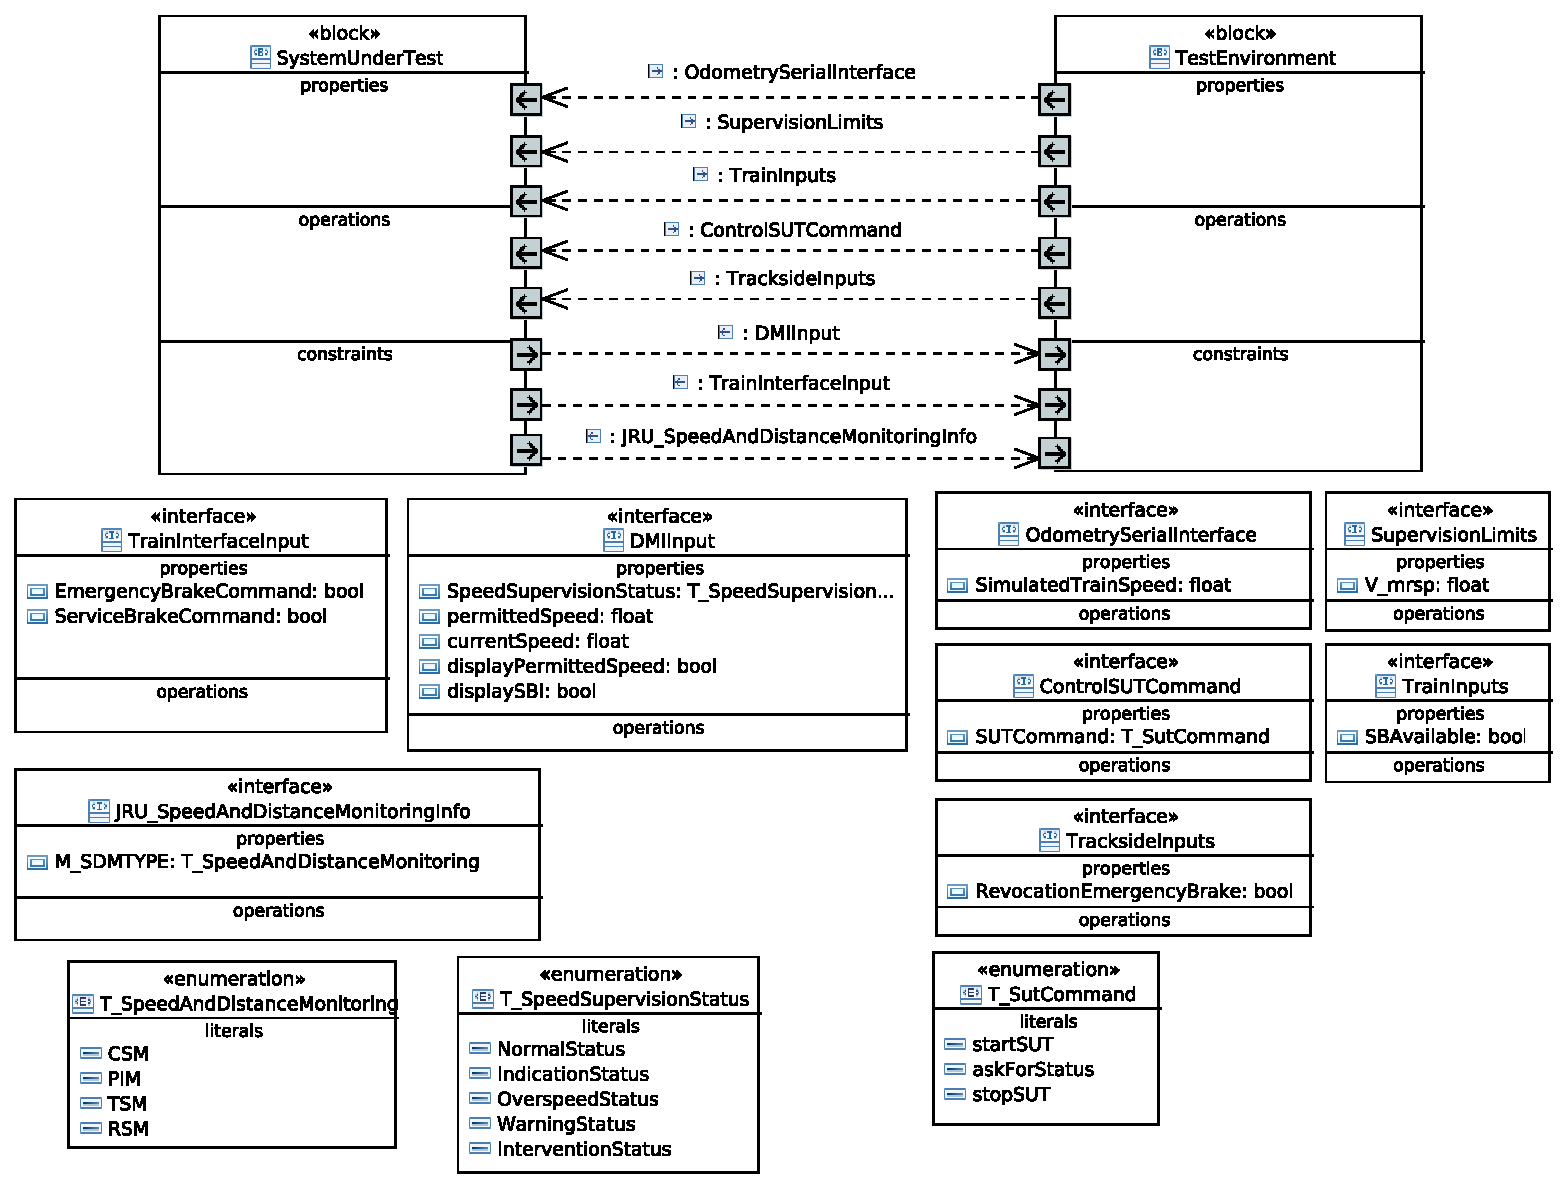
\includegraphics[width=\textwidth]{CSM-Interface.pdf} 
 %\vspace*{-5mm}
\caption{System interface of the ceiling speed monitor.}
 \label{fig:sysif}
 \end{figure}


 
Ceiling speed monitoring is activated and de-activated by the speed
and distance monitoring (SnD) coordination function that controls CSM,
TSM, and RSM: on input interface {\sf ControlSUTCommand}, variable $\csmsw$
specifies whether ceiling speed monitoring should be active
($\csmsw=\mathsf{startSUT}$) or passive, since target or release speed monitoring is
being performed ($\csmsw = \mathsf{stopSUT}$). 

The interface {\sf TrainInputs} carries
variable $\sbia$ which has value 1, if the train is equipped with a
service brake. This brake is then used for slowing down the train if
it has exceeded the maximal speed allowed, but not yet reached the
threshold for an emergency brake intervention. If $\sbia = 0$, the
emergency brake shall be used for slowing down the train in this
situation. Input $\sbia$ is to be considered as a configuration
parameter of the train, since it depends on the availability of the
service brake hardware. Therefore this value can be freely selected at
start-of-test, but must remain constant during test execution.

Input interface {\sf OdometrySerialInterface} provides the current
speed value estimated by the odometer equipment in variable
$\vest$. Input interface {\sf SupervisionLimits} provides the current
maximal velocity defined by the most restrictive speed profile in
variable $\vmax$. Input interface {\sf TracksideInput} provides a
control flag for the ceiling speed monitor: variable $\areb$ is 1, if
after an emergency brake intervention the brake may be automatically
released as soon as the estimated velocity of the train is again less
or equal to the maximal speed allowed. Otherwise ($\areb = 0$) the
emergency brakes must only be released after the train has come to a
standstill ($\vest = 0$).  This input parameter is a part of the
``national values'' given by the tracks, it may change when a train
crosses the boundaries between European countries, due to their local
regulations.

Output interface {\sf DMIInput} sends data from the SUT to the driver
machine interface (DMI). It carries five variables. $\dmicmd$ is used
to display the supervision status to the train engine driver: Value
{\sf IndicationStatus} may be initially present when CSM is activated,
but will be immediately overridden by one of the values {\sf
  NormalStatus}, {\sf OverspeedStatus}, {\sf WarningStatus}, or {\sf
  InterventionStatus}, as soon as ceiling speed monitoring becomes
active. Value {\sf NORMAL} is written by the SUT to this variable as long as
the ceiling speed is not violated by the current estimated
speed. Value {\sf OverspeedStatus} has to be set by the CSM as soon as
condition $\vmax < \vest$ becomes true. If the speed increases further
(the detailed conditions are described below), the indication changes
from {\sf OverspeedStatus} to {\sf WarningStatus}, and from there to
{\sf InterventionStatus}. The latter value indicates that either the
train is slowed down until it is back in the normal speed range, or
the emergency brake has been triggered to stop the train.
Furthermore, interface {\sf DMIInput} contains several speed-related
variables that are displayed on the DMI.





Output interface {\sf TrainInterfaceInput} specifies the train
interface from the CSM to the brakes, using variables $\ebcmd$ and
$\sbcmd$. If both equals $0$, both service
brakes (if existent) and emergency brakes are released. If $\sbcmd$ is
activated and $\ebcmd$ is not, the service brake is activated. If
$\ebcmd$ is activated, the emergency brake is
triggered.

Output interface {\sf JRU\_SpeedAndDistanceMoinitoringInfo} carries
the variable {\sf M\_SDMTYPE} that indicates which sub-function of the
speed and distance monitoring is active. 
The Juridical Recording Unit (JRU) is  used to record information
during the test phase, we have used this
interface as well as the DMI interface in compliance  with the testing
methodology defined by the European railway agency in \cite{ETCS-Subset076} (see section
\ref{sec:manualTest}).




% .......................................................................
\subsection{SUT Attributes and Operations}
The CSM executes sequentially; therefore 
the SUT block on the top-level interface diagram (Fig.~\ref{fig:sysif})  is refined 
to a single block representing the CSM,   as shown in Fig.~\ref{fig:sutcomposite}.
There, the SUT uses a local attribute $\sbicmd$ which 
carries value $1$, if the service
brake should be used for slowing down the train to the admissible
speed. If the value $0$ is assigned to 
$\sbicmd$, the emergency brake will be triggered in this situation.

\begin{figure}
%\hspace*{-50mm}
\centering
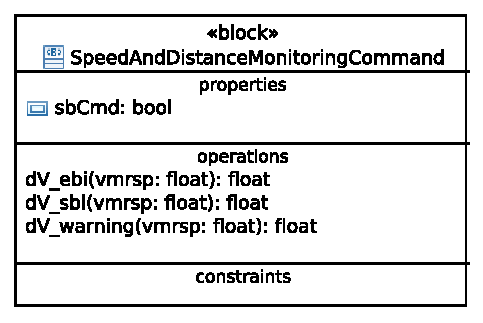
\includegraphics[]{CSM-SystemUnderTest.pdf}
%%\vspace*{-35mm}
\caption{Block diagram with CSM (sequential behaviour).}
 \label{fig:sutcomposite}
 \end{figure}


 
 
Three supervision limits are computed to assist the driver in
preventing automated service or emergency brake intervention by
maintaining the speed within certain limits, namely Warning, Service
brake intervention (sbi) and emergency brake intervention (ebi)
limits. These limits depend on the MRSP, and they are calculated
according to \cite{ETCSSRS-Principles} as follows.



 
\begin{equation}\label{eq:dvw}
\dvw(\vmax) = \left\{
\begin{array}{lc}
\min\{\frac{1}{3} + \frac{1}{30}\cdot\vmax,5 \}  &    \text{if}\ \ \vmax > 110 \\
4  &  \text{if}\ \ \vmax\le  110 \\
\end{array}
\right.
\end{equation}

\begin{equation}\label{eq:dvsbi}
\dvs(\vmax) = \left\{
\begin{array}{lc}
\min\{0.55+0.045\cdot\vmax,10 \}  &    \text{if}\ \ \vmax > 110 \\
5.5  &  \text{if}\ \ \vmax\le  110 \\
\end{array}
\right.
\end{equation}

\begin{equation}\label{eq:dvwe}
\dve(\vmax) = \left\{
\begin{array}{lc}
\min\{-0.75 + 0.075\cdot\vmax,15 \}  &    \text{if}\ \ \vmax > 110 \\
7.5  &  \text{if}\ \ \vmax\le  110 \\
\end{array}
\right.
\end{equation}

 


   
% .......................................................................
\subsection{CSM Behavioural Specification}
The behaviour of the ceiling speed monitor is modeled by a hierarchic state machine 
that is associated with the SUT block of Fig.~\ref{fig:sutcomposite}. The top-level machine (not shown here)
specifies the activation and de-activation of the CSM during the interplay between CSM, TSM, and RSM: state machine {\sf CSM\_ON} (this is the machine 
describing the behaviour of the CSM) is entered as soon as the value of 
input variable $\csmsw$ changes to {\sf startSUT}, and it is left when its value
changes to {\sf stopSUT}. 
The lower-level state machine  {\sf CSM\_ON}
models the behaviour of the active CSM, as displayed in Fig.~\ref{fig:csmsm}.

\begin{figure}
 \centering
%\hspace*{-15mm}
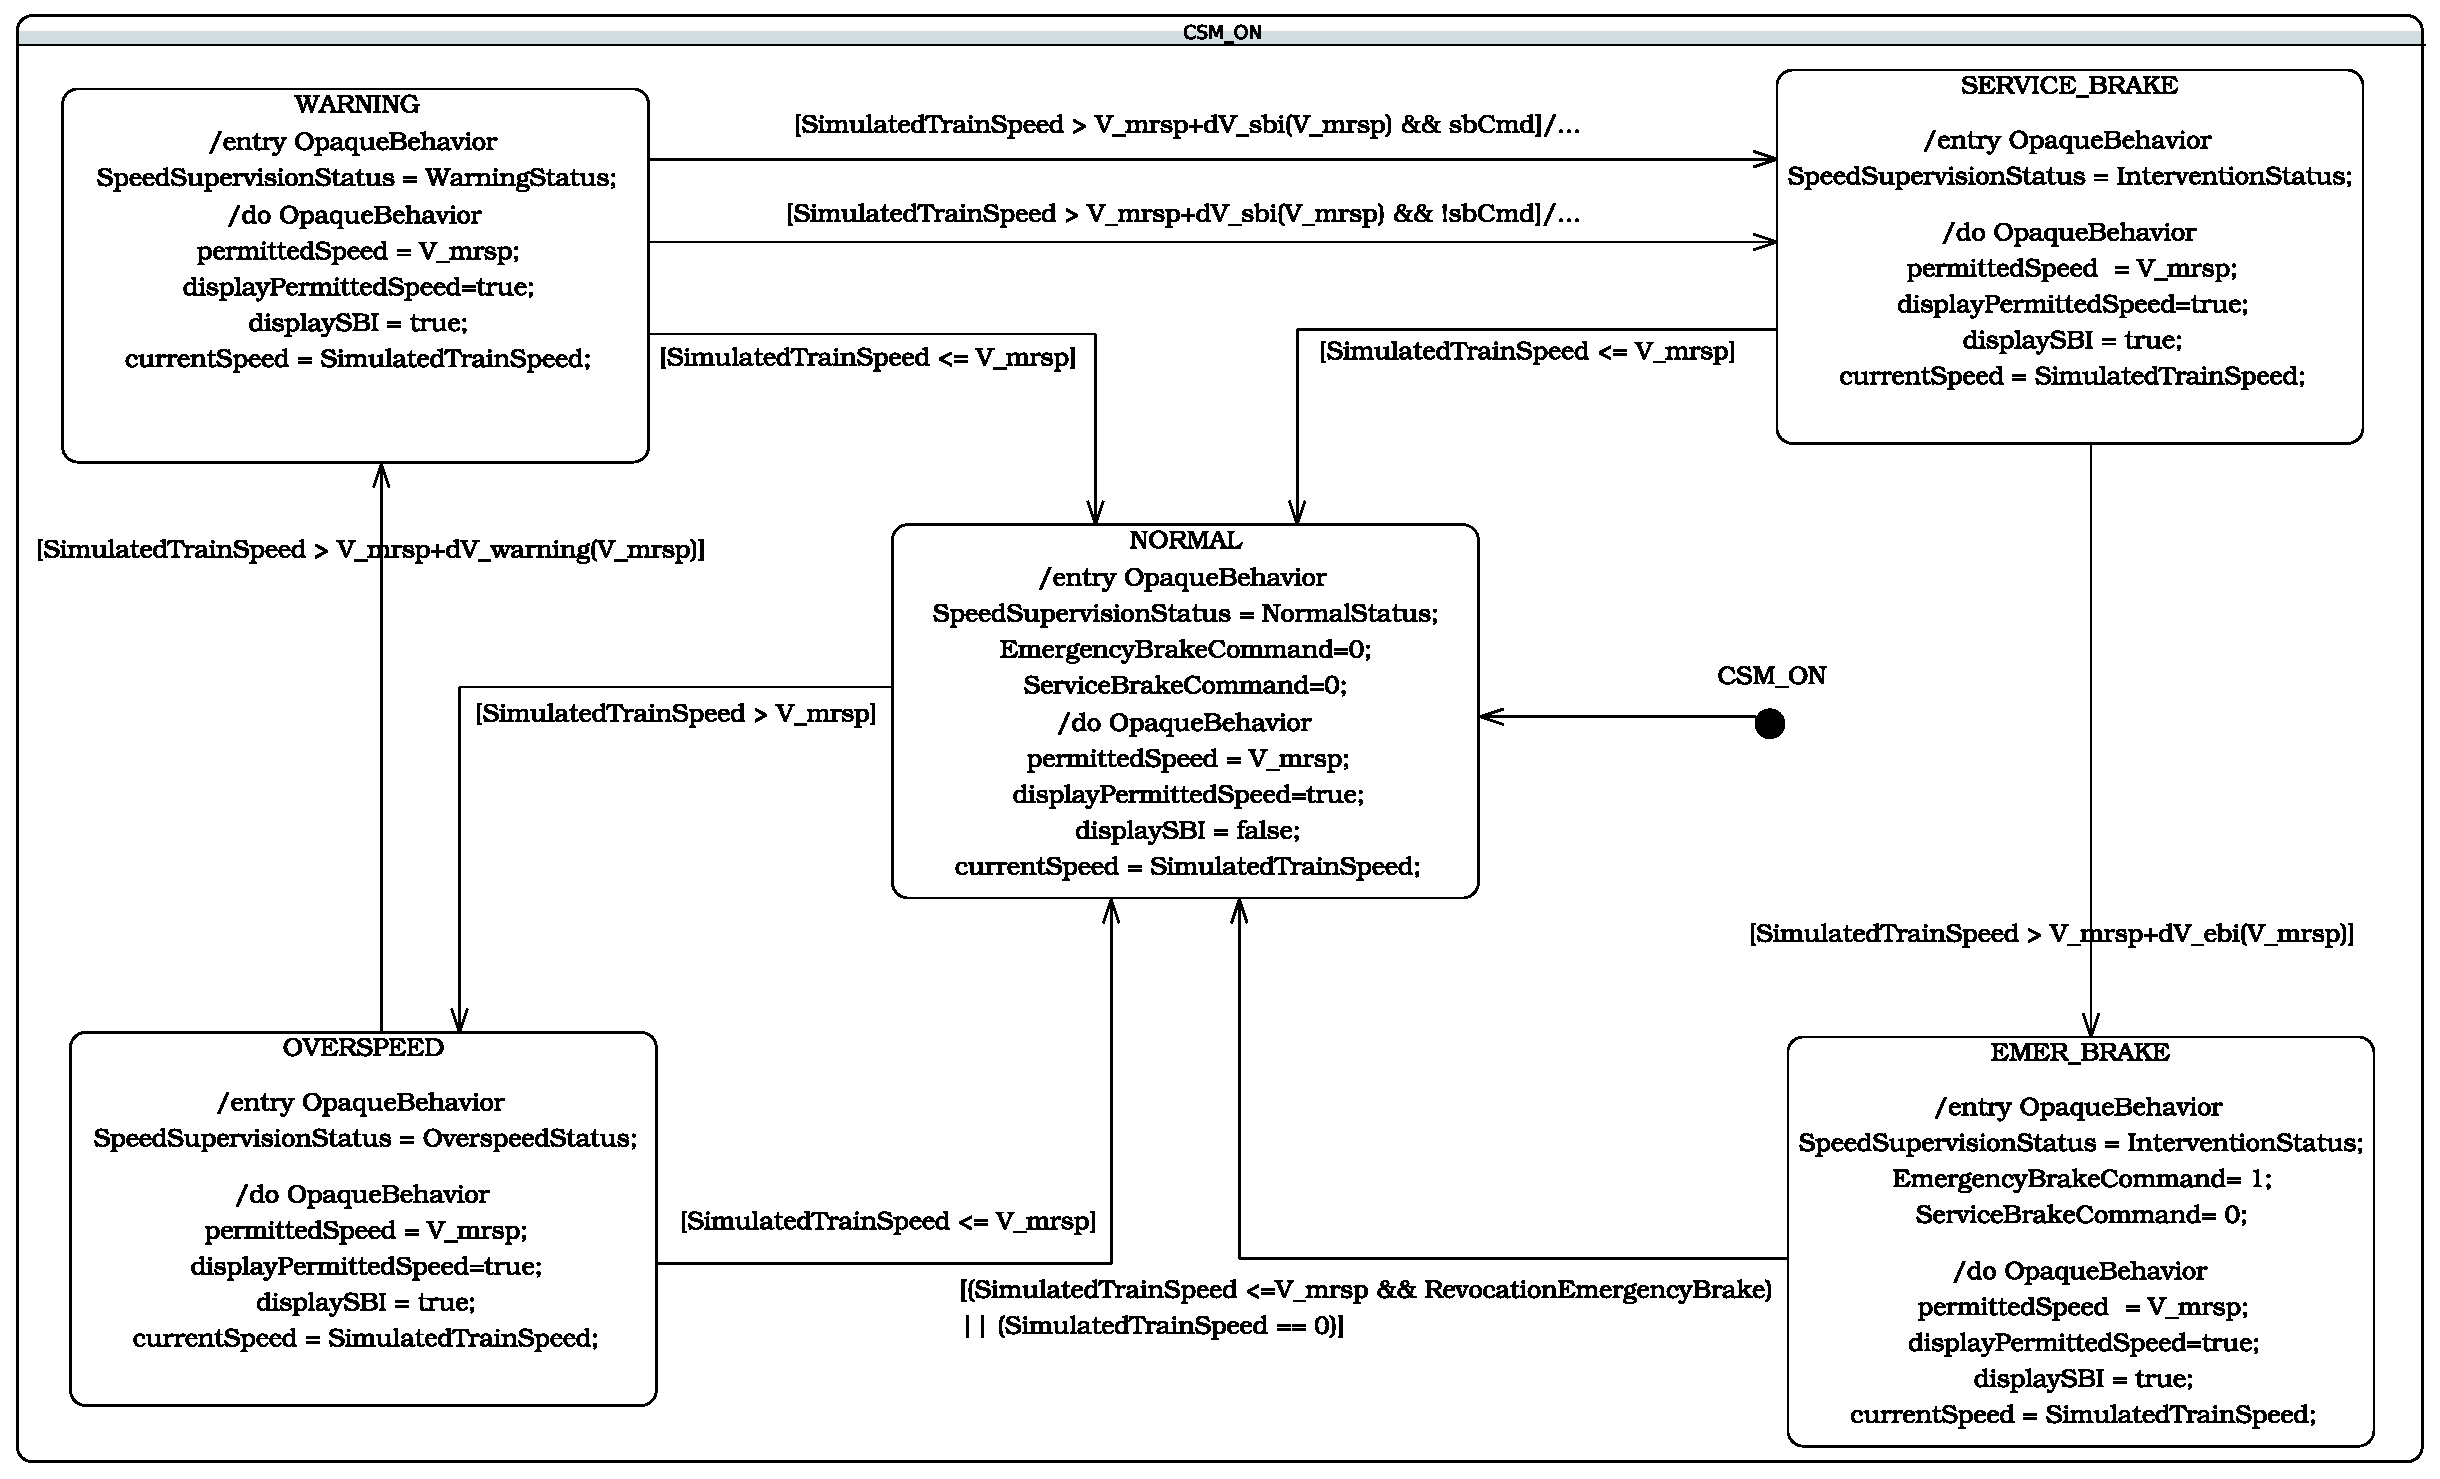
\includegraphics[width=\textwidth]{CSM-StateMachine.pdf}
%%\vspace*{-35mm}
\caption{Ceiling speed monitoring state machine.}
 \label{fig:csmsm}
 \end{figure}


Its execution starts in basic state {\sf NORMAL}, where the {\sf NormalStatus}
indication is displayed on the DMI and brakes are released 
($\ebcmd = 0$ and $\sbcmd = 0$). When the speed increases above the
maximal speed allowed ($\vest > \vmax$), the state machine transits to
basic state {\sf OVERSPEED}, where the {\sf OverspeedStatus} indication is displayed to the train engine driver. If the train continues over speeding until the warning threshold $\vmax + \dvw(\vmax)$ is exceeded, a transition
into the {\sf WARNING} state is performed, accompanied by an
indication change on the DMI. Accelerating further until $\vest >
\vmax + \dvs(\vmax)$ leads to a transition into basic state {\sf
  SERVICE\_BRAKE}, where either the service brake or the emergency
brake is triggered, depending on the value stored before in variable
$\sbicmd$. The DMI display changes to {\sf InterventionStatus}. 


 

The intervention status is realized by two basic state machine states, {\sf SERVICE\_BRAKE} and
{\sf EMER\_BRAKE}. From {\sf SERVICE\_BRAKE} it is still possible to return to {\sf NORMAL}, as soon as the speed has been decreased below the over speeding threshold. When the train, however, continues its acceleration until the emergency braking threshold has been exceeded ($\vest > \vmax+\dve(\vmax)$), basic state {\sf EMER\_BRAKE} is entered. From there, a state machine transition to {\sf NORMAL} is only possible if the train comes to a standstill, or if the national regulations (variable $\areb$)
allow to release the brakes as soon as over speeding has stopped.

Observe that the run-to-completion semantics of state machines also allows for zero-time
 transitions from, for example, {\sf NORMAL} to {\sf EMER\_BRAKE}. If,
 while in basic state {\sf NORMAL},  the inputs change such that
 $\vest > \vmax+\dve(\vmax)$ becomes true\footnote{This would be an
   exceptional behaviour situation, caused, for example, by temporary
   unavailability of odometry data, so that a ``sudden jump'' of
   $\vest$ would be observed by the CSM.}, the state machine
 transition from {\sf NORMAL} to {\sf OVERSPEED} leads to a transient
 model state, because guard condition $\vest > \vmax+\dvw(\vmax)$ is already
 fulfilled, and the state machine transits to {\sf
   WARNING}. Similarly, guards $\vest > \vmax+\dvs(\vmax)$ and $\vest >
 \vmax+\dve(\vmax)$ also evaluate to true, so that the next quiescent state
 is reached in basic state {\sf EMER\_BRAKE}.


% ============================================================
%%%@todo jp: add formal specification of the transition relation
% ============================================================

 



% .......................................................................
\subsection{Tracing Requirements to the Model}

SysML provides language elements for relating model elements to requirements, using the {\sf <<satisfy>>} relationship from model elements to requirements symbols in arbitrary SysML diagrams~\cite[Section~16]{SysML12}. Alternatively, SysML models may be augmented by
tables associating requirements and model elements. Exploiting this language feature supports both model validation and requirements-based testing.
In the former case, missing requirements can be detected if they
cannot be linked to structural or behavioural model elements in the
appropriate way. In latter case, execution traces through the model covering a
given structural or behavioural model element represent test cases
contributing to the verification of all requirements related to the
model element under consideration. 
%%%This technique is described in more detail below in Section~\ref{@todo}.
For the CSM model described above, the system requirements specified in 
Section~\ref{sec:sysreq} can be traced to model elements as follows.










\begin{table}[htbp]
\renewcommand{\arraystretch}{1.2}
\caption{Requirements links to the SysML
  Elements \label{table:req-tracing} }
\centering
\tabsize
\begin{tabular}{rrl}

\hline\hline
{\bf No.} & {\bf Requirement} & $\longleftarrow$ {\sf <<satisfy>>}
\\
\hline
1 &
REQ-3.13.10.2.1 & {\sf <<Composite State>>} {\sf CSM\_ON}  
\\\hline
2 &
REQ-3.13.10.2.2 & {\sf <<Transition>>} [{\sf EMER\_BRAKE} - {\sf NORMAL}]
\\ & &
{\sf <<Transition>>} [{\sf SERVICE\_BRAKE} - {\sf NORMAL}]
\\\hline
3 &
REQ-3.13.10.2.3 & {\sf <<Transition>>} [{\sf WARNING} - {\sf
SERVICE\_BRAKE}] ({\sf !sbCmd})
\\ & &
{\sf <<Basic State>>} {\sf SERVICE\_BRAKE}
\\\hline
4 &
REQ-3.13.10.2.4 & {\sf <<Transition>>} [{\sf EMER\_BRAKE} - {\sf NORMAL}]
\\ & &
{\sf <<Transition>>} [{\sf SERVICE\_BRAKE} - {\sf NORMAL}]
\\ & &
{\sf <<Transition>>} [{\sf WARNING} - {\sf SERVICE\_BRAKE}] ({\sf !sbCmd})
\\\hline
5 &
REQ-3.13.10.2.5 & {\sf <<Transition>>} [{\sf EMER\_BRAKE} - {\sf NORMAL}]
\\ & &
{\sf <<Transition>>} [{\sf SERVICE\_BRAKE} - {\sf NORMAL}]
\\\hline
6 &
REQ-3.13.10.3.1 & {\sf <<Submachine State>>} {\sf CSM\_ON}
\\\hline
7 &
REQ-3.13.10.3.2 & {\sf <<Basic State>>} {\sf OVERSPEED}  
\\ & &
{\sf <<Basic State>>} {\sf SERVICE\_BRAKE}  
\\ & &
{\sf <<Basic State>>} {\sf WARNING}  
\\ & &
{\sf <<Basic State>>} {\sf EMER\_BRAKE} 
\\\hline
8 &
REQ-3.13.10.3.3 .r0 & {\sf <<Transition>>} [{\sf EMER\_BRAKE} - {\sf NORMAL}]
\\
 & .r1 & {\sf <<Transition>>} [{\sf OVERSPEED} - {\sf NORMAL}]
\\ & &
{\sf <<Transition>>} [{\sf SERVICE\_BRAKE} - {\sf NORMAL}]
\\ & &
{\sf <<Transition>>} [{\sf WARNING} - {\sf NORMAL}]
\\ & &
{\sf <<Transition>>} [{\sf EMER\_BRAKE} - {\sf NORMAL}]
\\  & .t1 & {\sf <<Basic State>>} {\sf NORMAL}  
\\  & .t2 & {\sf <<Basic State>>} {\sf OVERSPEED}  
\\  & .t3 & {\sf <<Basic State>>} {\sf WARNING}  
\\  & .t4 & {\sf <<Basic State>>} {\sf SERVICE\_BRAKE}  
\\  & .t5 & {\sf <<Basic State>>} {\sf EMER\_BRAKE}  
\\\hline
9 & REQ-3.13.10.3.4 .r1c2 & {\sf <<Constraint>>} constraint\_14
\\ & .r1c3 & {\sf <<Transition>>} [{\sf OVERSPEED} - {\sf NORMAL}]
\\ & .r1c4 & {\sf <<Transition>>} [{\sf WARNING} - {\sf NORMAL}]
\\ & .r1c5 & {\sf <<Transition>>} [{\sf EMER\_BRAKE} - {\sf NORMAL}]
\\ & & {\sf <<Transition>>} [{\sf SERVICE\_BRAKE} - {\sf NORMAL}]
\\ & .r3c1 & {\sf <<Transition>>} [{\sf NORMAL} - {\sf OVERSPEED}]
\\ & .r3c2 & {\sf <<Constraint>>} constraint\_15
\\ & .r4c1 & {\sf <<Constraint>>} constraint\_08 
\\ & .r4c2 & {\sf <<Constraint>>} constraint\_16 
\\ & .r4c3 & {\sf <<Transition>>} [{\sf OVERSPEED} - {\sf WARNING}]
\\ & .r5c1 & {\sf <<Constraint>>} constraint\_10 
\\ & & {\sf <<Constraint>>} constraint\_09 
\\ & .r5c2 & {\sf <<Constraint>>} constraint\_17
\\ & .r5c3 & {\sf <<Constraint>>} constraint\_12 
\\ & & {\sf <<Constraint>>} constraint\_11 
\\ & .r5c4 & {\sf <<Transition>>} [{\sf WARNING} - {\sf SERVICE\_BRAKE}]
\\ & &
{\sf <<Transition>>} [{\sf SERVICE\_BRAKE} - {\sf EMER\_BRAKE}]
\\ & &
{\sf <<Constraint>>} constraint\_13 
\\\hline
10 &
REQ-3.13.10.3.5 & {\sf <<Constraint>>} constraint\_05 
\\ & &
{\sf <<Constraint>>} constraint\_06 
\\ & &
{\sf <<Constraint>>} constraint\_07 
\\ & &
{\sf <<Basic State>>} {\sf NORMAL} 
\\ & &
{\sf <<Constraint>>} constraint\_04 
\\\hline
11 &
REQ-3.13.10.3.6 & {\sf <<Constraint>>} constraint\_05 
\\ & &
{\sf <<Constraint>>} constraint\_06 
\\ & &
{\sf <<Constraint>>} constraint\_07 
\\ & &
{\sf <<Constraint>>} constraint\_04 

\\
\hline\hline
\end{tabular}

%%%@todo Modify run-to-completion/stability constraints

\end{table}


Tables \ref{table:req-tracing} associates 
the SysML elements with the requirements they satisfiy.  ``Submachine
State'' and  ``Atomic State'' refer to the top-level states of composite
machines and to basic control states, respectively. 
%% The ``Constraints" refer to
%% temporal logic formulas specified in LTL that are used to
%% relate the most complex requirements to execution traces as explained in Section~\ref{@todo}.
 

The complexity of {\sf <<satisfy>>} relations between structural or behavioural model elements depends on the complexity of the requirement and the way it is reflected by the structural and behavioural model. Consider, for example (see Table~\ref{tab:req}), requirement  
\begin{itemize}
\item REQ-3.13.10.2.1: The train speed indicated to the driver shall be identical to the speed used for the speed monitoring (i.e. the estimated speed $\vest$).
\end{itemize}

Every model trace where the CSM is activated is suitable for verifying this requirement, because the DMI variable $\std$ is updated by the actual speed $\vest$ via operation $\calcstd$, whenever the ceiling speed monitor is active, that is, in composite state {\sf CSM\_ON}. Therefore 
{\sf CSM\_ON} is linked to REQ-3.13.10.2.1 by the {\sf <<satisfy>>} relation, as expressed
in Table~\ref{table:req-tracing}, row~1. 

 


A more complex case of requirements tracing presents itself if one or more transitions are related to a given requirement. This is the case for the requirement
\begin{itemize}
\item REQ-3.13.10.2.2: Once a Train Interface command (traction cut-off, service brake or emergency brake) is triggered, the on-board shall apply it until its corresponding revocation condition is met.
\end{itemize}

As modeled in Fig.~\ref{fig:csmsm}, we have two revocation conditions; one is reflected by the transition from basic state {\sf SERVICE\_BRAKE} to {\sf NORMAL}, the other from {\sf EMER\_BRAKE} to {\sf NORMAL}. Therefore both transitions are related to REQ-3.13.10.2.2, as specified in row~2 of Table~\ref{table:req-tracing}.
In the  most complex case we have to handle situations where requirements are reflected by traces visiting model state {\it vectors}\footnote{A model state vector consists of valuations of  inputs, outputs, and internal model variables, as well as of variable valuations indicating the basic state machine states currently active.} fulfilling certain constraints, and these model state vectors have to be visited by the traces in a specific order. Such a situation is reflected, for example, by 
\begin{itemize}
\item REQ-3.13.10.3.4:
The on-board equipment shall execute the transitions between the different supervision statuses as described in Table~\ref{tab:seven} (see~\cite[4.6.1]{ETCSSRS-Principles} for details about the symbols). This table takes into account the order of precedence between the supervision statuses and the possible updates of the MRSP while in ceiling speed monitoring (e.g. when a TSR is revoked; TSR = Temporary Speed Restriction).
\end{itemize}


This requirement may be decomposed into atomic sub-requirements one
for each pertinent cells of table \ref{tab:six}.  Some of these
sub-requirements are again reflected by transitions. Sub-requirement
REQ-3.13.10.3.4.r5c1, however, specifies the possibility to directly
transit from {\sf NORMAL} to {\sf SERVICE\_BRAKE} or {\sf
  EMER\_BRAKE}. This cannot be specified by simply linking a
behavioural model element to the sub-requirement, because we have avoided
to draw direct state machine transitions from {\sf NORMAL} to {\sf
  SERVICE\_BRAKE} or {\sf EMER\_BRAKE}, since those transitions are
implicitly realized by the run-to-completion semantics, as explained
above. In the formalization of requirements tracing described in
Section~\ref{sec:formaltrc} we show how these situations can be
covered by using traceability specifications by means of temporal
logic formulas.

















\section{Requirements Driven Approach}
\label{sec:req}
\subsection{Formal Requirements Tracing in SysML Models}
\label{sec:formaltrc}
% ============================================================================


%@todo jp: Describe how requirements are formally reflected by sets of computations, and how these sets can be specified by means of LTL safety formulas and revise the 
%following paragraphs


Consider, for example, the zero-time transition
{\sf NORMAL} $\trans$ {\sf SERVICE\_BRAKE}. To cover this situation, we need to 
\begin{enumerate}
\item Enter   {\sf NORMAL} in a quiescent model state -- this is specified by 
$$[\mathsf{NORMAL} \wedge \vest \le \vmax]$$
\item Stay there until the speed exceeds $\vmax + \dvs(\vmax)$ but remains less or equal to $\vmax+\dve$.
\end{enumerate}
Formally this is expressed in LTL by 
\[
\begin{array}{l}
 \mathsf{Finally} ([\mathsf{NORMAL}\wedge \vest \le \vmax]  \wedge {}
 \\\tabf
 ([\mathsf{NORMAL}\wedge \vest \le \vmax]
 \\\tabf \ \
 \mathsf{Until}
 \\\tabf\
 [\mathsf{NORMAL}\wedge \vest > \vmax+\dvs(\vmax) \wedge {}
 \\\tabf \  \
 \vest \le \vmax+\dve(\vmax)]))
\end{array}
\]
This is expressed by constraint\_09 linked to REQ-3.13.10.3.4.r5c1 in Table~\ref{table:req-tracing}.
%% and specified in Table~\ref{tab:constraints}.
Similarly, covering the zero-time transition {\sf NORMAL} $\trans$ {\sf EMER\_BRAKE} requires a trace satisfying
\[
\begin{array}{l}
 \mathsf{Finally} ([\mathsf{NORMAL}\wedge \vest \le \vmax]  \wedge {}
 \\\tabf
 ([\mathsf{NORMAL}\wedge \vest \le \vmax]
 \\\tabf \ \
 \mathsf{Until}
 \\\tabf\
 [\mathsf{NORMAL}\wedge \vest > \vmax+\dve(\vmax)]))
\end{array}
\]
%% (this is specified as constraint\_10 in Table~\ref{tab:constraints}).
Similar constraints are specified for 
REQ-3.13.10.3.4.r1c2,
REQ-3.13.10.3.4.r3c2,
REQ-3.13.10.3.4.r4c1,
REQ-3.13.10.3.4.r4c2,
REQ-3.13.10.3.4.r5c2,
REQ-3.13.10.3.4.r5c3 and 
REQ-3.13.10.3.4.r5c4
as well as for requirements REQ-3.13.10.3.5 and REQ-3.13.10.3.6.


%% \begin{table}
%% \caption{Constraints related to complex requirements listed in Table~\ref{table:req-tracing}.}
%% \begin{center}
%% \scriptsize
%% \hspace*{-10mm}
%% \begin{tabular}{|l|p{12cm}|}
%% \hline\hline
%% {\sf <<Constraint>>} & {\bf LTL Formula}
%% \\\hline\hline
%% constraint\_01 & 
%% \parbox{120mm}{
%% \vspace*{1mm}
%% $\mathbf{Finally} [\mathsf{EMER\_BRAKE} \wedge \neg \sbia \wedge 
%%          \vest > 0 \wedge \vest \le  \vmax \wedge\neg  \areb]$ 
%% \vspace*{1mm}         
%% }
%% \\\hline
%% constraint\_02 &  
%% \parbox{120mm}{
%% \vspace*{1mm}
%% $\mathbf{Finally} [\mathsf{SERVICE\_BRAKE} \wedge\neg\sbia \wedge\vest\le\vmax]$
%% \vspace*{1mm}
%% }
%% \\\hline
%% constraint\_03 &  
%% \parbox{120mm}{
%% \vspace*{1mm}
%% $\mathbf{Finally} [\mathsf{SERVICE\_BRAKE} \wedge\neg\sbia\wedge \vest > \vmax + \dvs(\vmax) \wedge \vest \le \vmax + \dve(\vmax)]$
%% \vspace*{1mm}
%% }
%% \\\hline
%% constraint\_04 & 
%% \parbox{120mm}{
%% \vspace*{1mm}
%% $\mathbf{Finally} [\mathsf{CSM\_OFF} \wedge \csmsw \wedge \vest > \vmax  \wedge \vest \le \vmax + \dvw(\vmax) ]$
%% \vspace*{1mm}
%% } 
%% \\\hline
%% constraint\_05 &
%% \parbox{120mm}{
%% \vspace*{1mm}
%% $\mathbf{Finally} [\mathsf{CSM\_OFF} \wedge\csmsw \wedge \vest > \vmax + \dvw(\vmax) \wedge \vest\le\vmax+\dvs(\vmax) ]$
%% \vspace*{1mm}
%% }  
%% \\\hline
%% constraint\_06 & 
%% \parbox{120mm}{
%% \vspace*{1mm}
%% $\mathbf{Finally} [\mathsf{CSM\_OFF} \wedge\csmsw\wedge \vest > \vmax + \dvs(\vmax) \wedge \vest \le \vmax + \dve(\vmax) ]$
%% \vspace*{1mm}
%% } 
%% \\\hline
%% constraint\_07 &  
%% \parbox{120mm}{
%% \vspace*{1mm}
%% $\mathbf{Finally} [\mathsf{CSM\_OFF} \wedge\csmsw\wedge \vest > \vmax + \dve(\vmax) ]$
%% \vspace*{1mm}
%% }
%% \\\hline
%% constraint\_08 &  
%% \parbox{120mm}{
%% \vspace*{1mm}
%% $\mathbf{Finally} ([\mathsf{NORMAL} \wedge \vest\le\vmax] \wedge  
%% ([\mathsf{NORMAL} \wedge  \vest\le\vmax]\ \mathbf{Until}\ [\mathsf{NORMAL} \wedge \vest > \vmax + \dvw(\vmax) \wedge \vest\le\vmax + \dvs(\vmax) ]))$
%% \vspace*{1mm}
%% }
%% \\\hline
%% constraint\_09 &  
%% \parbox{120mm}{
%% \vspace*{1mm}
%% $\mathbf{Finally} ([\mathsf{NORMAL} \wedge \vest\le\vmax] \wedge  
%% ([\mathsf{NORMAL} \wedge  \vest\le\vmax]\ \mathbf{Until}\ [\mathsf{NORMAL} \wedge \vest > \vmax + \dvs(\vmax) \wedge \vest\le\vmax + \dve(\vmax) ]))$
%% \vspace*{1mm}
%% }
%% \\\hline
%% constraint\_10 &  
%% \parbox{120mm}{
%% \vspace*{1mm}
%% $\mathbf{Finally} ([\mathsf{NORMAL} \wedge \vest\le\vmax] \wedge  
%% ([\mathsf{NORMAL} \wedge  \vest\le\vmax]\ \mathbf{Until}\ [\mathsf{NORMAL} \wedge \vest > \vmax + \dve(\vmax)]))$
%% \vspace*{1mm}
%% }
%% \\\hline
%% constraint\_11 &  
%% \parbox{120mm}{
%% \vspace*{1mm}
%% $\mathbf{Finally} ([\mathsf{OVERSPEED} \wedge \vest\le\vmax] \wedge  
%% ([\mathsf{OVERSPEED} \wedge  \vest\le\vmax]\ \mathbf{Until}\ [\mathsf{OVERSPEED} \wedge \vest > \vmax + \dvs(\vmax) \wedge \vest\le\vmax + \dve(\vmax) ]))$
%% \vspace*{1mm}
%% }
%% \\\hline
%% constraint\_12 &  
%% \parbox{120mm}{
%% \vspace*{1mm}
%% $\mathbf{Finally} ([\mathsf{OVERSPEED} \wedge \vest\le\vmax] \wedge  
%% ([\mathsf{OVERSPEED} \wedge  \vest\le\vmax]\ \mathbf{Until}\ [\mathsf{OVERSPEED} \wedge \vest > \vmax + \dve(\vmax)]))$
%% \vspace*{1mm}
%% }
%% \\\hline
%% constraint\_13 &  
%% \parbox{120mm}{
%% \vspace*{1mm}
%% $\mathbf{Finally} ([\mathsf{WARNING} \wedge \vest\le\vmax] \wedge  
%% ([\mathsf{WARNING} \wedge  \vest\le\vmax]\ \mathbf{Until}\ [\mathsf{WARNING} \wedge \vest > \vmax + \dve(\vmax)]))$
%% \vspace*{1mm}
%% }
%% \\\hline
%% constraint\_14 &  
%% \parbox{120mm}{
%% \vspace*{1mm}
%% $\mathbf{Finally} ([\mathsf{M\_SDMTYPE != CSM} \ \wedge \ 
%% {\sf IndicationStatus}] \mathbf{Until}\ 
%% [\mathsf{M\_SDMTYPE != CSM} \ \wedge \  {\sf IndicationStatus} ] \wedge
%% \mathsf{SUTCommand} \ \wedge \ \vest \leq \vmax ])$
%% \vspace*{1mm}
%% }
%% \\\hline
%% constraint\_15 &  
%% \parbox{120mm}{
%% \vspace*{1mm}
%% $\mathbf{Finally} ([\mathsf{M\_SDMTYPE != CSM} \ \wedge \ 
%% {\sf IndicationStatus}] \mathbf{Until}\ 
%% [\mathsf{M\_SDMTYPE != CSM} \ \wedge \  {\sf IndicationStatus} ] \wedge
%% \mathsf{SUTCommand} \ \wedge \ \vest > \vmax \ \wedge \ \vest \leq \vmax + \dvw(\vmax) ])$
%% \vspace*{1mm}
%% }
%% \\\hline
%% constraint\_16 &  
%% \parbox{120mm}{
%% \vspace*{1mm}
%% $\mathbf{Finally} ([\mathsf{M\_SDMTYPE != CSM} \ \wedge \ 
%% {\sf IndicationStatus}] \mathbf{Until}\ 
%% [\mathsf{M\_SDMTYPE != CSM} \ \wedge \  {\sf IndicationStatus} ] \wedge
%% \mathsf{SUTCommand} \ \wedge \  \vest > \vmax
%% + \dvw(\vmax) \ \wedge \ \vest \leq \vmax + \dvs(\vmax)])$
%% \vspace*{1mm}
%% }
%% \\\hline
%% constraint\_17 &  
%% \parbox{120mm}{
%% \vspace*{1mm}
%% $\mathbf{Finally} ([\mathsf{M\_SDMTYPE != CSM} \ \wedge \ 
%% {\sf IndicationStatus}] \mathbf{Until}\ 
%% [\mathsf{M\_SDMTYPE != CSM} \ \wedge \  {\sf IndicationStatus} ] \wedge
%% \mathsf{SUTCommand} \ \wedge \  \vest > \vmax
%% + \dvs(\vmax) ])$
%% \vspace*{1mm}
%% }
%% \\\hline

%% \hline
%% \end{tabular}
%% \normalsize
%% \end{center}
%% \label{tab:constraints}
%% \end{table}%















% =============================================================================


\subsection{Manually Defined Tests}
\label{sec:manualTest}
The European Railway agency provides a test specification
\cite{ETCS-Subset076} along with the requirements of the EVC.  The
tests aim at verifying the conformity and the functionality of the onboard 
subsystems against the system requirement specification (SRS)
\cite{ETCS}.  The SRS has been decomposed into a set of features such
that a feature groups a set of requirements that can be tested at the
available interfaces. The test cases have been designed to ensure that
a test of a given feature is independent of all other
feature. Moreover tests are only described as a reaction to a given
stimulation at the interface of the feature.

The test specification formalises the test cases
description, each test case is composed of
\begin{itemize}
\item  a unique identifier,
\item  a short description of the target of the test,
\item  a list of covered requirement,
\item an initial state of the test e.g. initial assignment to the
internal test variables,
\item the test  steps:  inputs change and expected outputs, and
\item a final test state e.g. initial assignment to the
internal test variables.
\end{itemize}


Table~\ref{tbl:manualtest} summarizes the available
tests. The second column describes the objective of each test.  The
column ``Covers Requirements'' shows the list of requirements covered
by the tests. We have refined the list provided by the standard. We
first refer to the sub-requirement when needed and secondly, we add
some requirements that are covered by side effect  to be able to
provide more accurate requirement coverage.

The ceiling speed monitoring feature is associated with 8 test cases
in~\cite{ETCS-Subset076}.  They cover the change of the speed
supervision status and the brake commands depending on  the train
speed. We only use seven of them (TC-CSM-[1-7]), the one missing
covers a requirement that we assume, is “delegated” to the surrounding software
of the CSM.
Eight test cases cover the general requirement of the speed and
distance monitoring feature in~\cite{ETCS-Subset076}. Four of those
are test cases outside the scope of the ceiling speed monitoring and
therefore not included in our benchmark.
The four others cover the requirements {\sf REQ-3.13.10.2.3} and
{\sf REQ-3.13.10.2.4} but only in the target speed monitoring section. We
have adapted them to fit into the collection of CSM tests. Moreover,
we grouped them in pairs (TC-GR-[1-2]) . Each pair is dealing with two different ways
of receiving inputs depending on the  ERTMS mode that is not
relevant for testing the CSM function.


\begin{table}
\tabsize
\renewcommand{\arraystretch}{1.2}
\caption{Test cases from the Subset 076}
\label{tbl:manualtest}
\begin{tabular}{lp{.48\textwidth}p{4.9cm}}
\hline\hline
Identifier & Target of the test & Covered Requirements \\
\hline
TC-CSM-1 & 
When the train runs in CSM  and does not exceed the
the permitted speed, no intervention is triggered and the 
{\sf NormalStatus} is displayed.& 
REQ-3.13.10.3.1, REQ-3.13.10.3.3,\newline
REQ-3.13.10.3.5 \\ \hline
TC-CSM-2 & 
When the train runs in CSM and the speed is between the permitted
speed and the Warning limit, no intervention is triggered and the 
{\sf OverspeedStatus} is displayed. Once the train speed is below 
the permitted speed the {\sf NormalStatus} is displayed. & 
REQ-3.13.10.3.1, REQ-3.13.10.3.2,\newline
REQ-3.13.10.3.3, REQ-3.13.10.3.4 \\ \hline
TC-CSM-3 & 
When the train runs in CSM and the speed is between the Warning limit
speed and the SBI supervision limit, no intervention is triggered and the 
{\sf WarningStatus} is displayed. Once the train speed is below 
the permitted speed the {\sf NormalStatus} is displayed. & 
REQ-3.13.10.3.1, REQ-3.13.10.3.2, \newline
REQ-3.13.10.3.3, REQ.3.13.10.3.4.r4 \\ \hline
TC-CSM-4 & 
When the train runs in CSM and the speed is between the SBI
supervision limit and
the EBI supervision limit , the service brake intervention is triggered and the 
{\sf InterventionStatus} is displayed. Once the train speed is below 
the permitted speed the {\sf NormalStatus} is displayed. & 
REQ-3.13.10.2.2, REQ-3.13.10.3.1,\newline
REQ-3.13.10.3.2, REQ-3.13.10.3.3,\newline 
REQ-3.13.10.3.4 \\ \hline
TC-CSM-5 & 
When the train runs in CSM and the speed is greater then 
the EBI supervision limit , the emergency brake intervention is triggered and the 
{\sf InterventionStatus} is displayed. Once the train reaches
standstill the {\sf NormalStatus} is displayed. & 
REQ-3.13.10.2.2, REQ-3.13.10.2.5, \newline
REQ-3.13.10.3.1, REQ-3.13.10.3.2, \newline
REQ-3.13.10.3.3, REQ-3.13.10.3.4 \\ \hline
TC-CSM-6 & 
When entering CSM mode the Indication status is overwritten &
REQ-3.13.10.3.1, REQ-3.13.10.3.3,\newline
REQ-3.13.10.3.4, REQ-3.13.10.3.6 \\ \hline
TC-CSM-7 & 
When the train is between the permitted speed and the Warning limit
the  SBI  supervision limit also referred
as the FLOI (First Line Of Intervention) is 
displayed. Once the train speed is below 
the permitted speed the {\sf NormalStatus} is displayed  & 
REQ-3.13.10.3.1, REQ-3.13.10.3.2,\newline
REQ-3.13.10.3.3, REQ-3.13.10.3.4, \newline
REQ-3.13.10.3.5\\ \hline
TC-GR-1 & 
When the use of service brake is not allowed the emergency brake
command shall be triggered instead. The emergency brake is then revoked
according to the service brake revocation.& 
REQ-3.13.10.2.1, REQ-3.13.10.2.3,\newline
REQ-3.13.10.2.4, REQ-3.13.10.3.3,\newline
REQ-3.13.10.3.4 \\ \hline
TC-GR-2 & 
The use of service brake is not allowed and the train exceeds the EBI
supervision limit, the emergency brake command shall be triggered. 
The emergency brake is then revoked only when the train reaches
standstill.&
REQ-3.13.10.2.1, REQ-3.13.10.2.3,\newline
REQ-3.13.10.2.4, REQ-3.13.10.3.3,\newline
REQ-3.13.10.3.4 \\ 
\hline\hline
\end{tabular}
\normalsize
\end{table}




These 9 test cases has been translated into LTL formula to fit our
experiments platform. This translation is performed by representing
the steps by a sequence of nested until operator.
Let the test sequence be of the following form: $i_0,i_1,o_0,i_2, o_1,o_2$ where
$i_k$ ($o_k$) represents an input (resp. output) assignment to an interface
variables. The associated LTL formula will be in the following form:\\
$$ \mathsf{Finally}( [i_0 \wedge i_1 \wedge o_0] \wedge ([i_0 \wedge i_1 \wedge
o_0] \; \mathsf{Until} \;[i_2 \wedge \mathsf{Finally}([o_1 \wedge o_2]) ) $$
Intuitively the inputs are set and do not change until a new input configuration
is reached and implies new  output values.

\begin{figure}
\begin{Verbatim}[numbers=left]
TC-CSM-2;
 Finally ([currentSpeed > 0 && 
           currentSpeed < V_mrsp &&
           SpeedSupervisionStatus == NormalStatus && 
           displayPermittedSpeed == 1 ]
          &&
          ([currentSpeed > 0 && 
            currentSpeed < V_mrsp &&
            SpeedSupervisionStatus == NormalStatus && 
            displayPermittedSpeed == 1 ]
          Until
          (([currentSpeed > V_mrsp && 
             currentSpeed <= V_mrsp + dV_Waring(V_mrsp)]  && 
             Finally[
                     SpeedSupervisionStatus ==  OverspeedStatus && 
                     displayPermittedSpeed == 1 && 
                     displaySBI == 1 && 
                     ServiceBrakeCommand == 0 ])
              &&
              ([currentSpeed > V_mrsp  && 
                currentSpeed <= V_mrsp + dV_Waring(V_mrsp) ]   
              Until
              ([currentSpeed > 0 && currentSpeed < V_mrsp ] &&
                Finally[SpeedSupervisionStatus == NormalStatus ])))));

\end{Verbatim}
\caption{Example of test case TC-CSM-2 as LTL formula\label{fig:testltlex}}
\end{figure}

Figure \ref{fig:testltlex} shows the LTL formula used to represent the
test case TC-CSM-2. 
\begin{itemize}
\item lines 2-5~: The train is moving within the permitted speed and
the DMI aspects is coherent with the normal status.
\item lines 7-13~: The train stays in the initial configuration until
the speed is greater than permitted speed but below the Warning limit.
\item lines 14-21~: The DMI information changes according to the new
speed.
\item line 23~: The train speed is now back below the permitted.
\item line 24~: The Normal status is now displayed.
\end{itemize}



%%  LocalWords:  EVC EBI WarningStatus InterventionStatus SBI CSM FLOI  REQ
%%  LocalWords:  DMI

\subsection{Extended Manually Defined Tests}
\label{sec:extendedManualTest}
The test specification provided by the European Railway agency (\cite{ETCS-Subset076})
contains test suites for the different ETCS features. The sub-requirements
REQ-3.13.10.3.4.r1c2, REQ-3.13.10.3.4.r3c2, REQ-3.13.10.3.4.r4c2 and REQ-3.13.10.3.4.r5c2
describe a transition from supervision status \emph{Indication} to \emph{Normal}, \emph{Overspeed}, \emph{Warning} and \emph{Intervention}.
Supervision status \emph{Indication} is not used by CSM, but requirement
REQ-3.13.10.3.6 states, that if CSM is ativated with supervision status
being \emph{Indication}, the state changes shall occur as defined in the
sub-requirements above.
The manual test case for REQ-3.13.10.3.6 defined in \cite{ETCS-Subset076}
only covers the state transition from \emph{Indication} to \emph{Normal}.
Therefore the test manual test suite does not cover the sub-requirements
REQ-3.13.10.3.4.r3c2, REQ-3.13.10.3.4.r4c2 and REQ-3.13.10.3.4.r5c2.

Our analysis shows that the sub-requirements REQ-3.13.10.3.4.r5c3 and
REQ-3.13.10.3.4.r5c4 are not covered by the tests defined in \cite{ETCS-Subset076}.
These two sub-requirements define the behaviour of CSM with
supervision status being \emph{Overspeed} and the trigger conditions
require to directly change to \emph{Intervention} (REQ-3.13.10.3.4.r5c3) and
supervision status being \emph{Warning} and the trigger conditions
require to change to \emph{Intervention} (REQ-3.13.10.3.4.r5c4).

To be able to compare the test manually defined suite with automatically
generated test suites presented in \ref{sec:automated_ETCS_test} and the equivalence class testing
approach presented in \ref{sec:ecpt}, additional test procedure have manually been added
to cover the missing requirements\footnote{See table \ref{tbl:extendedmanualtest}}.

\begin{table}
\tabsize
\renewcommand{\arraystretch}{1.2}
\caption{Additional test cases to cover the remaining sub-requirements.}
\label{tbl:extendedmanualtest}
\begin{tabular}{lp{.37\textwidth}p{6.4cm}}
\hline\hline
Identifier & Target of the test & Covered Requirements \\
\hline
TC-CSM-8 & 
When entering CSM mode the Indication status is overwritten &
REQ-3.13.10.3.4.r1c2, REQ-3.13.10.3.4.r3c2,\newline
REQ-3.13.10.3.4.r4c2, REQ-3.13.10.3.4.r5c2,\newline
REQ-3.13.10.3.6 \\ \hline
TC-CSM-9 & 
Switching from \emph{Overspeed} to \emph{Intervention} and \emph{Warning} to \emph{Intervention}&
REQ-3.13.10.3.4.r5c3, REQ-3.13.10.3.4.r5c4 \\
\hline\hline
\end{tabular}
\normalsize
\end{table}

\subsection{Automatically Defined Tests}
\label{sec:automated_ETCS_test}
% ===========================================================
%%@todo jp: check adjustments from uwe
% ===========================================================

The CSM model described in Section~\ref{chap:model} contains
requirement tracing information. Instead of manually translating the
test cases specified for the CSM feature into LTL formulas
\footnote{as described in the previous section \ref{sec:manualTest}},
the requirement tracing information from the model can be
used to automatically generate test procedures covering these
requirements.
%% The tracing information in the test model
%% and the test cases for the feature CSM are both based on the same
%% requirement specification of the CSM feature. In both cases
%% knowledge about the system and understanding of the requirements
%% has been used to interpret the requirement and define tracing
%% information. The difference is where and how the
%% generated tracing information is represented and how it can be used further.
%% When creating the model, the tracing information was directly defined
%% as part of the model in form of SysML satisfy relations.
%% This also allows to review the correctness of this tracing
%% information directly in the test model.
In this section, we describe how the requirement tracing information
defined in the model can be used to automatically generate test
procedures for full requirements coverage from the CSM model.
Note that the test procedures in section \ref{sec:manualTest} also are
automatically generated test procedures providing requirements coverage,
but they have been generated from a manually developed formal test
case specification. The approach presented here uses the requirement
tracing information defined in the model to automatically generate
the formal test case specification and in a second step to
automatically generate the test procedures covering these test cases.
Through this, a test suite is generated in a fully automated way
that covers all requirements represented in the model.

The test generation tool from our experiments platform automatically
generates test cases for different kinds of model coverage strategies
from a test model\footnote{More detailed explanation on the coverage criteria may be found in \cite{D34.1}.}:
\begin{itemize}
\item {\bf Basic Control State Coverage (BCS)}\newline
      This type of behavioural coverage aims at covering each
      basic control state of each state machine at least once.
      No additional objectives are made about concurrent control
      states or accompanying variable valuations when reaching
      the control state under consideration.
\item {\bf Transition Coverage (TR)}\newline
      Transition coverage aims at covering each transition of
      every state machine in the model. Again, no restrictions
      are made regarding variable valuations, control states
      and concurrent transitions to be performed when the one
      under consideration is triggered.
\item {\bf MC/DC Transition Coverage (MCDC)}\newline
      Modified condition/decision (MC/DC) coverage is a variant
      of transition coverage, where non-atomic guard conditions
      are evaluated in a systematic manner.
\item {\bf Hierarchic Transition Coverage (HITR)}\newline
      For a transitions emanating from higher-level control states,
      different underlying basic control states can be active when
      the transition is triggered. Hierarchic transition coverage
      aims at exercising these transitions once for every underlying
      basic control state being active.
\item {\bf Basic Control States Pair Coverage (BCSPAIR)}\newline
      For concurrent state machines pairs of states of two
      different state machines have to be active simultaneously.
      This strategy does not apply to the test model under consideration,
      because it does not contain concurrent state machines.
      \footnote{This coverage criteria does not apply to the CSM
      test model described in chapter \ref{chap:model}, as it
      does not include concurrent state machines.}
%% \item {\bf User Defined LTL Specification (UD)}\newline
%%      For each LTL constraint that is linked to a system component
%%      and that satisfies a requirement, a test case is generated
%%      using the LTL constraint as the test goal.
\end{itemize}

The test model contains requirements together with satisfy relations
linking them to model elements. These requirements are taken directly
from the ETCS specification (\cite{ETCS}).
The requirements 3.13.10.3.3 and 3.13.10.3.4 have been
refined into sub-requirements to allow better tracing to model elements
and to be able to define the requirements coverage in more detail.
%% Therefore, the test model contains \numsubreq{} requirements which can be
%% traced back to the \numreq{} requirements defined for the ceiling speed
%% monitoring feature of ETCS.
Satisfy relations are defined in the model that link transitions,
basic control states or LTL-formulas to requirements.
The test generation tool automatically generates test cases that
cover states, transitions or user defined LTL constraints with
the different test strategies described above.
The satisfy relations defined in the
model are used to determine the set of automatically generated
test cases that satisfy a requirement.
A requirement is covered if the respective set of the automatically
generated test cases (generated from the model) has been covered.

\begin{table}
\caption{Model Derived Requirements Coverage Tests}\label{tbl:derivedtest}
\tabsize
\centering
\begin{tabular}{p{40mm}p{30mm}r}
\hline\hline
Test Procedure Name & Requirements & Number of Test Cases\\
\hline
TP-REQ-3.13.10.2.1 & REQ-3.13.10.2.1 & 1\\
TP-REQ-3.13.10.2.2 & REQ-3.13.10.2.2 & 2\\
TP-REQ-3.13.10.2.3 & REQ-3.13.10.2.3 & 10\\
TP-REQ-3.13.10.2.4 & REQ-3.13.10.2.4 & 3\\
TP-REQ-3.13.10.2.5 & REQ-3.13.10.2.5 & 2\\
TP-REQ-3.13.10.3.1 & REQ-3.13.10.3.1 & 2\\
TP-REQ-3.13.10.3.2 & REQ-3.13.10.3.2 & 18\\
TP-REQ-3.13.10.3.3 & REQ-3.13.10.3.3 & 24\\
TP-REQ-3.13.10.3.4 & REQ-3.13.10.3.4 & 16\\
TP-REQ-3.13.10.3.5 & REQ-3.13.10.3.5 & 6\\
TP-REQ-3.13.10.3.6 & REQ-3.13.10.3.6 & 4\\
\hline\hline
\end{tabular}
\end{table}

For each of the requirements from the ETCS specification, one
test procedure has been generated that covers all automatically generated
test cases that satisfy the requirement (or any of its sub-requirements).
Whether it is possible to completely
cover a requirement in a single test procedure and how well
requirement can be represented in a test model highly depends on
the requirements and on the test model. In this case, we were able
to link all requirements
\footnote{All requirements under consideration that are relevant for ceiling speed monitoring}
from the ETCS specification to
test model elements and to automatically generate a test suite
that provides full requirements coverage.
Table \ref{tbl:derivedtest} also provides the number of test cases that
are covered during the test procedure and that are necessary
to test the requirement. Naturally test cases can occur in multiple
test procedures.



\newcommand{\q}{\textbf{q}}

\section{Improving Tests through Equivalence Class Testing Strategy}\label{sec:ecpt}
\label{sec:ecpt}

 In~\cite{peleska_sttt_2014}, two of the authors have presented a novel complete 
input equivalence class partition (IECP) testing strategy. In \cite{peleska_csm_2014}
this approach has first been applied to the Ceiling Speed Monitor and the analysis of
manually created mutants indicated that this strategy is superior to model derived test cases relying on
structural criteria of the state machine. In \cite{huebner15} the approach was evaluated 
with automatically generated mutants from a Java implementation. Here different refinements of
the strategy were compared and evaluated. For the Ceiling Speed Monitor a mutation score of 100 \%
could be achieved using a combination of equivalence class testing and boundary value tests.  



%@todo: copied from TAP publication, update the following sections for journal
%version

\subsection{Semantic Domain.} 

The novel equivalence class partition testing strategy presented 
in~\cite{peleska_sttt_2014} is applicable to deterministic, livelock-free systems 
with conceptually infinite input domains and finite internal state and output domains.
``Conceptually infinite'' means that the domains are too large to be explicitly 
enumerated for test purposes. This includes physical models with real-valued inputs,
but can also apply to finite but very large data types such as 64 bit integers or
doubles as used in typical programming languages or modelling formalisms. As pointed out 
in~\cite{peleska_sttt_2014,peleska_csm_2014}, this class of systems is quite
significant in the embedded systems domain: typical candidates are controllers 
processing analogue inputs and deriving discrete control decisions from these inputs, such
as thrust reversal controllers in aircrafts, or the speed monitors and airbag controllers described
in this paper.

The strategy has been proven to  be complete on the semantic domain of \emph{Reactive Input Output State Transition Systems (RIOSTS)} ${\cal S} = (S,s_0,R,V,D)$. These systems have state spaces $S$,
initial state $s_0\in S$, and transition relations $R\subseteq S\times S$. Their state spaces
consist of valuation functions $s: V\fun D$, where $V$ is a set of variable symbols and $D$ is 
the union of all variable domains. The variable symbols can be partitioned into $V = I\cup M \cup O$,
where $I$ comprises input variables, $M$ (internal) model variables, and $O$ output variables.
RIOSTS distinguish between \emph{quiescent} states $s\in S_Q$ and \emph{transient} states $s'\in S_T$,
such that $S_Q\cup S_T$ partitions the state space $S$. Transitions from quiescent states only change
input valuations, while internal model variables and output variables remain unchanged. The
resulting post-states may be quiescent or transient. Transitions from transient states always have
uniquely determined quiescent post-states (so we only allow deterministic RIOSTS here), and the associated transitions  leave the inputs
unchanged. This concept represents a natural abstraction of timed formalisms, where 
delay transitions allow for time to pass and inputs to be changed, while discrete
transitions produce output and change internal state, but are executed in zero 
time~\cite[p.~687]{DBLP:books/daglib/0020348}.

By associating atomic propositions $AP$ with free variables in $V$, any RIOSTS can be extended to a 
Kripke Structure~\cite{clarke_em-etal:1999a} 
$K({\cal S}) = (S,s_0,R,V,D,L,AP)$. The labelling function $L:S\fun 2^{AP}$
maps $s\in S$ to the set of all atomic propositions $p\in AP$ that evaluate to $\ist$,
when replacing every free variable $v$ of $p$ by its valuation $s(v)$ in state $s$.

\paragraph{Notation.}
In the exposition below, variable symbols are enumerated with the naming conventions
   $I = \{ x_1,\dots,x_k\}$, $M = \{m_1,\dots, m_p\}$, $O = \{y_1,\dots,y_q\}$. We use   notation
$\vec x = (x_1,\dots,x_k)$  for input variable vectors, and their   valuation in state $s$ is written as $s(\vec x) = (s(x_1),\dots,s(x_k))$. $D_I = D_{x_1}\times\dots\times D_{x_k}$ denotes the Cartesian product of the input variable domains. Tuples $\vec m, \vec y$ and $D_M$ and $D_O$ are defined over model variables and outputs in an analogous way. By $s\oplus\{\vec x \mapsto \vec c\}, \ \vec c \in D_I$ we denote the state $s'$ which coincides with $s$ on all variables from $M\cup O$, but maps the input vector to valuation $s'(\vec x) = \vec c$. 
For $(s_1,s_2)\in R$ we also use the shorter expression $R(s_1,s_2)$.  Restricting a state $s$ to variable symbols from a set $U \subseteq V$ is denoted by $s|_U$. This function has domain $U$ and coincides with $s$ on this domain.

% --------------------------------------------------------------------------
\subsection{Application to Concrete Modelling Formalisms.} 
The test strategy described below is elaborated on the semantic domain of RIOSTS. Every concrete
modelling formalism whose behavioural semantics can be represented by RIOSTS is automatically 
equipped with such a test strategy: the concrete model $M$ is translated into its corresponding RIOSTS ${\cal S}$. Then the test strategy is applied to ${\cal S}$, and this results in a set of test cases, each case represented by a finite sequence of inputs to the SUT. When executing the test cases, 
the transition relation of ${\cal S}$ is used to determine whether the SUT's reactions to these
input sequences are adequate. In this article, concrete models are expressed by SysML state machines,
and these can be associated with RIOSTS semantics which is consistent with the semi-formal specification of state machine behaviour in the UML/SysML standards~\cite{uml_2_4,SysML12}.




% --------------------------------------------------------------------------
\subsection{Equivalence Classes.}
We use the term {\it trace} to denote finite sequences of states, input vectors, or output vectors.
Applying a trace $\iota = \vec c_1\dots\vec c_n$ 
of input vectors $\vec c_i\in D_I$ to an RIOSTS ${\cal S} = (S,s_0,R,V,D)$  residing in some quiescent state
$s\in S$ stimulates a sequence of state transitions, each pair of consecutive states
connected by the transition relation $R$, and with associated  output changes  
as triggered by these inputs. 
Restricting this   sequence to quiescent states, this results in
a trace of states
$\tau = s_1.s_2\dots s_n$ such that $s_i(\vec x) = \vec c_i, i = 1,\dots,n$, and
$s_i(\vec y)$ is the last STS output resulting from application of $\vec c_1\dots\vec c_i$ 
to state $s$.\footnote{Observe that the restriction to quiescent states does not result in a loss
of information. Every transient state has the internal and output variable valuations coinciding with its quiescent pre-state, and its input valuation is identical to that of its quiescent
post-state.} This trace $\tau$ is  denoted by $s/\iota$. The restriction of $s/\iota$ to output variables is denoted by the trace $(s/\iota)|_O$.
Since transient states have unique quiescent post-states, $(s/\iota)|_O$ is a uniquely determined
output trace.
Two quiescent states $s, s'$ are {\it I/O-equivalent}, written $s\sim s'$, 
if every non-empty input trace $\iota$, when applied to $s$ and $s'$, results in the same outputs, that is,  
$(s/\iota)|_O = (s'/\iota)|_O$. Two STS ${\cal S}, {\cal S}'$ with the same input domain are I/O-equivalent, if their initial states 
are I/O-equivalent.
Note that  $s\sim s'$ asserts equivalent I/O-behaviour {\it in the future}, while it still admits that states $s$ and $s'$ show different output valuations, i.e.~$s|_O \neq s'|_O$. 
 

Since I/O-equivalence  $\sim$ is an equivalence relation on quiescent states, 
we can factorise $S_Q$ with respect to  $\sim$.
The \emph{initial input equivalence class partitioning (IECP)} ${\cal I}\subseteq\mathbb{P}(D_I)$ 
associated with $S_Q/_\sim$ is 
the coarsest partitioning of $D_I$ such that for all $\q\in S_Q/_\sim$, $X\in {\cal I}$,
there exists a uniquely determined I/O-equivalence class $ \delta(\q,X)\in S_Q/_\sim$, 
such that
\begin{equation}\label{eq:iecpa}
 \forall s\in \q, \vec c\in X: s/\vec c \in \delta(\q,X)
\end{equation}
and there exists a well-defined output $\omega(\q,X)\in D_O$, such that
\begin{equation}\label{eq:iecpb}
\forall s\in \q, \vec c\in X: (s/\vec c)|_O =  \omega(\q,X)
\end{equation}
It is shown in~\cite{peleska_sttt_2014} that $S_Q/_\sim$ is finite
 if the RIOSTS ${\cal S}$
has finite internal state domains and finite output domains, while the input domains may be infinite.
Moreover,   the coarsest partitioning ${\cal I}$  exists, and it is finite and uniquely determined under these prerequisites.
For these RIOSTS, 
properties (\ref{eq:iecpa}) and (\ref{eq:iecpb}) induce an abstraction    
  to DFSMs   
with state space $S_Q/_\sim$, input alphabet ${\cal I}$, and output alphabet
$D_O$:  (\ref{eq:iecpa})
specifies a well-defined total transition function $\delta : S_Q/_\sim\times {\cal I} \fun S_Q/_\sim$, and (\ref{eq:iecpb}) a well-defined
output function $\omega : S_Q/_\sim\times {\cal I} \fun D_O$.
When partitioning ${\cal I}$ further to a refined IECP $\overline{\cal I}$,
the characteristic properties (\ref{eq:iecpa}),(\ref{eq:iecpb}) are preserved.  

A finite sequence $X_1\dots X_k, X_i\in{\cal I}$   is called an \emph{abstract test case}:
concrete test input vectors $\vec c_i$  can be selected from each $X_i$, and, when applied
to the initial state $s_0$, this selection induces a trace $s_1\dots s_k$ of 
quiescent states, such that
$$
\exists \q_1,\dots,\q_k\in  S_Q/_\sim:\forall i \in \{ 1,\dots,k \}: 
s_i\in \q_i\wedge \q_i = \delta(\q_{i-1},X_i)
$$
The IECP properties imply that the
\emph{expected results} associated with this test case are then specified by the
output trace $\omega(\q_{i-1},X_i), i=1,\dots,k$.


 

In~\cite{peleska_sttt_2014} an algorithm for calculating  $S_Q/_\sim$ and ${\cal I}$ is given.
This algorithm produces propositions over variables from $V$, 
specifying the members of $S_Q/_\sim$ and ${\cal I}$, respectively. Making use of an SMT solver, the algorithm allows for identifying the  reachable I/O-equivalence classes
 $\q \in S_Q/_\sim$. As a consequence, every proposition characterising an abstract test
 case $X_1\dots X_k$  is actually feasible: this means that we can find concrete
traces in ${\cal S}$ such that, after deleting the transient states, the resulting
quiescent state sequence $s_0.s_1\dots s_k$ fulfils $s_i\in\q_i$ for $i = 0,\dots,k$ 
and $s(\vec x)\in X_i$ for $i = 1,\dots,k$.

For the model described in section~\ref{chap:model}, input equivalence
classes are unions of convex subsets of $\mathbb{R}^n$. It should be noted, however, that the
notion of I/O-equivalence and IECPs introduced here is far more general, since arbitrary propositional specifications of I/O-equivalence classes can be handled by the 
underlying theory. The input equivalence classes identified in~\cite[Example~1]{peleska_sttt_2014}, for example, contain members 
$z$ specified by conditions $z\!\! \mod m = n$.




% --------------------------------------------------------------------------
\subsection{Fault Models.}
%Complete black box test strategies are typically defined with respect to a given fault model 
%${\cal F} = ({\cal S},\sqsubseteq,{\cal D})$: ${\cal S}$ is the reference model 
%representing the ideal SUT behaviour. Relation $\sqsubseteq$ is a conformance relation describing
%the acceptable SUT behaviours,  so that an SUT whose behaviour is represented by some  
%${\cal S}'$ shall be accepted if and only if ${\cal S}' \sqsubseteq {\cal S}$.
%The fault domain ${\cal D}$ specifies a set of models that may or may not conform to ${\cal S}$,
%and it is assumed that the true behaviour of the SUT is identical to that of an   ${\cal S}'$
%contained in ${\cal D}$.

For the semantic domain of RIOSTS,
the fault models ${\cal F} = ({\cal S},\sim,{\cal D}({\cal S},m,\overline{{\cal I}}))$ are specified as follows.
The reference models ${\cal S}$ are semantic RIOSTS representations  of models elaborated in concrete formalisms, such that the expected behaviour of the SUT is specified by ${\cal S}$ up to 
I/O-equivalence. We use  I/O-equivalence as conformance relation.


Positive integer $m$ fulfils   
$m\ge n$, where $n$ is the number of I/O-equivalence classes of ${\cal S}$.
IECP $\overline{{\cal I}}$ is a refinement of the initial coarsest IECP ${\cal I}$  associated with ${\cal S}$.
Then the
  members ${\cal S}'$ of the fault domain ${\cal D}({\cal S},m,\overline{{\cal I}})$ 
are RIOSTS specified as follows.
\begin{enumerate}
\item The states of ${\cal S}'$ are defined over the same I/O variable space $ I \cup O$ as defined for the model ${\cal S}$.

\item Initial state $s_0'$ of ${\cal S}'$ coincides with initial state 
$s_0$ of ${\cal S}$ on $I\cup O$. 

\item ${\cal S}'$ generates only finitely many different output values. 

\item ${\cal S}'$ has a well-defined reset operation allowing to re-start the system from its initial state.

\item The number of I/O-equivalence classes of ${\cal S}'$ is less or equal $m$.
 


\item
\label{item:adequacy}  If ${\cal I}$, ${\cal I}'$ are the initial coarsest IECP of  ${\cal S}$, ${\cal S}'$, respectively, 
fulfilling the characteristic properties~(\ref{eq:iecpa}), (\ref{eq:iecpb}), then 
$\overline{{\cal I}}$ fulfils
  the following \emph{adequacy condition}: 
\begin{equation}\label{eq:x2}
\begin{array}{l}
\forall X\in {\cal I}, X'\in {\cal I}':  
\big(X\cap X'\neq\varnothing \Rightarrow
\exists \overline{X}\in \overline{{\cal I}}: \overline{X} \subseteq X\cap X'\big)
\end{array}
\end{equation}


\end{enumerate}



The intuition behind the adequacy condition~\ref{item:adequacy} is as follows. Every possible behaviour of a fault domain member ${\cal S}'$ can be exercised by visiting a state in 
some I/O-equivalence class $\q'$ and applying an input of some IECP member $X'\in {\cal I}'$
to this state. Using the refined IECP $\overline{{\cal I}}$ in the test suite as described below,
ensures that an input from $\overline{X}\subseteq X'\in {\cal I}'$ will be selected when 
${\cal S}'$ resides in $\q'$, so the behaviour associated with $(\q',X')$ will be stimulated in
at least one of the test cases. If,  when in a 
state of $\q'$,  ${\cal S}'$
conforms to the behaviour of ${\cal S}$ for all inputs from $X \setminus X'$, but fails
for inputs from $X\cap X'$, inputs selected from $\overline{X}\subseteq X\cap X'$ will uncover this error.

Conversely, suppose now that
 the reference model  ${\cal S}$ behaves differently, when IECs $X_1, X_2\in {\cal I}$
are applied in some state $\q$. Suppose further that ${\cal S}'$ fails to make this case 
distinction in a corresponding state $\q'$. Then there exists $X'\in {\cal I}'$ such that
 ${\cal S}'$ shows the same behaviour for all $\vec c\in X'$, but $X_1\cap X'\neq \varnothing$
 and $X_2\cap X'\neq \varnothing$, so two different behaviours should be visible according
 to the reference model. Now the adequacy condition guarantees that there exist two IEC
$\overline{X}_1, \overline{X}_2\in \overline{{\cal I}}$, such that 
$\overline{X}_1\subseteq X_1\cap X'$ and 
$\overline{X}_2\subseteq X_2\cap X'$.
 As a consequence, if inputs from every input class 
of $\overline{{\cal I}}$ are exercised, the behavioural differences for inputs from
$X_1\cap X'$ and $X_2\cap X'$ will be revealed. Summarising, the adequacy condition ensures that 
the IECP $\overline{{\cal I}}$ from where input data to the SUT is selected is fine-grained 
enough to stimulate every possibly deviating behaviour of ${\cal S}$ and ${\cal S}'$. These facts
are exploited in the complete test strategy described next.
 
 
 

% ==========================================================================
\subsection{Complete Finite Test Suite.}

The complete DFSM abstraction ${\cal M}$
 of ${\cal S}$ with states $S_Q/_\sim$, input alphabet
 $\overline{{\cal I}}$, transition function and output function
  as characterised in (\ref{eq:iecpa}), (\ref{eq:iecpb}), allows for application of 
finite complete DFSM testing strategies, such as the \emph{W-Method} introduced 
in~\cite{chow:wmethod,vasilevskii1973}. 
The general form of a W-Method test suite is 
\begin{equation}\label{eq:wtestsuite}
{\cal W} = P.\big(\bigcup_{i=0}^{m-n}\overline{\cal I}^i.W\big)
\end{equation}
where $P$ is the state transition cover, $\overline{\cal I}^i$ denotes the input trace segments of length $i$, and $W$ is the characterisation set.  Every test of  ${\cal W}$ consists of a (possibly empty) input trace from $P$, concatenated with an arbitrary input trace of length zero up to $m-n$, and  terminated by an input trace from the characterisation set. 
$P$  is the union of a {\it state cover} $C$ and  a
{\it transition cover} 
$C.\overline{\cal I}$: $C$ contains   the empty trace $\varepsilon$,
 and for any state $\q$ of ${\cal M}$, there exists an input trace in $C$ which, 
 when applied to the initial state, ends at $\q$. The transition cover  
 is defined by 
 $C.\overline{\cal I}=\{\iota.X~|~\iota \in C, X\in \overline{\cal I}\}.$ Summarising, the input sequences of a state transition cover ensure that (1) every state of the reference 
DFSM ${\cal M}$ associated with the reference model ${\cal S}$ is visited, and (2) every transition from every state is exercised.    A characterisation set is a set of input traces distinguishing each pair of states in a minimal DFSM. Using minimisation algorithms such as the one specified in~\cite{gill62}, characterisation sets can be constructed as a by-product of the minimisation process.

The test suite generated according to (\ref{eq:wtestsuite}) is called an 
\emph{abstract test suite}, because its elements are abstract test cases as defined above:
the inputs to be used in each test case are not yet
represented by concrete input vectors $\vec c$, but by input equivalence classes 
$\overline{X}\in \overline{{\cal I}}$. For creating an executable test suite,  inputs
$\vec c\in \overline{X}$ have to be selected for every   
$\overline{X}\in\overline{{\cal I}}$. 

The W-Method is complete for the fault model of all DFSM over the
same input and output alphabet and with at most $m$ states. It is shown in~\cite{peleska_sttt_2014}
that the associated   test suites with concrete inputs $\vec c\in \overline{X}$ are also complete for 
${\cal F} = ({\cal S},\sim,{\cal D}({\cal S},m,\overline{{\cal I}}))$. This completeness 
result is independent on the choice of concrete input data selected from each input 
equivalence class $X\in\overline{\cal I}$.

The fault domain ${\cal D}({\cal S},m,\overline{{\cal I}})$ introduced above
can be extended by increasing $m$ or by refining $\overline{{\cal I}}$. Increasing
$m$ increases the maximal length of input sequences in test cases in a linear way.
This affects the size of the test suite exponentially, 
but allows for fault domain members with 
higher \emph{recurrence diameters} $r$~\cite{biere_linear_2006}: 
this is the length of the longest loop-free path in
a Kripke structure. Erroneous SUT behaviour that only occurs at the end of such a longest loop 
free path may only be detected if the test cases use input sequences that are long enough
to traverse the SUT state up to the length of the recurrence diameter. 

Refining $\overline{{\cal I}}$ increases the size of the IECP, and this size 
increases the number of test cases in a polynomial way. It has to be noted, however,
that uniformly refining all members of $\overline{{\cal I}}$ -- for example, by using 
a sub-paving strategy as it is well known from interval analysis~\cite{jaulin2001} -- increases the size of the IECP exponentially with each new refinement step. 
The resulting fault domain contains members ${\cal S}'$ 
possessing narrower \emph{trapdoors}: these
are refined input guard conditions $g\wedge \delta$ applicable in certain ${\cal S}'$-states,
where  ${\cal S}'$ should behave uniformly for all inputs satisfying $g$. 
The true behaviour of ${\cal S}'$, however, 
conforms to the expected behaviour modelled by ${\cal S}$ only for inputs
fulfilling $g\wedge \neg\delta$, while   erroneous behaviour is revealed for inputs 
satisfying $g\wedge \delta$.

\subsection{Refinement and Randomisation of Equivalence Partition Tests}\label{sec:ecpt:refinement}
%\subsection{Randomisation of Equivalence Partition Tests}\label{sec:randomisation}

As we have seen above, the fault domain ${\cal D}({\cal S},m,\overline{{\cal I}})$ can be enlarged
via $m$ or $\overline{{\cal I}}$. As a drawback this seriously affects the size of the
resulting complete test suite ${\cal W}$. Therefore a refinement of the input equivalence 
class partitioning $\overline{{\cal I}}$ should be used which effectively increases the resulting 
test suites ability to uncover faults. In \cite{huebner15} two refinement heuristics were investigated and it could be
shown that these heuristics are able to improve the test strength of the resulting test suite.
Basically these two improvements work as follows:

\begin{enumerate}
  \item An input partitioning $\overline{\cal I}$ is used. $\overline{\cal I}$ is a refinement of the initial coarsest IECP and
reflects all case distinctions visible in guard conditions.
\item Additionally all boundary value conditions can be used in order to generate boundary
value tests of the original equivalence classes
\footnote{This can be done by adding extra constraints defining the
  boundaries of the original equivalence classes. As an example
  consider the guard condition $x\leq n$ restricting the input
  variable $x$ in input equivalence class $\overline{X}\in
  \overline{\cal I}$ to values less or equal $n$. In this case the
  additional constraint $\gamma$ defined as $x=n$ yields two new
  equivalence classes $\overline{X}_\gamma\subset\overline{X} $ and
  $\overline{X}_{\neg\gamma}\subset\overline{X}$ with
  $\overline{X}_{\gamma}\cap
  \overline{X}_{\neg\gamma}=\emptyset$. $\overline{X}_{\gamma}$ is the
  set of input vectors $\vec c_{\overline{X}_\gamma}$ that fulfill
  $x=n$ and thus are the boundaries of the original equivalence class
  $\overline{X}$ containing all input vectors, where $x<n$ or $x=n$.}.
\end{enumerate}


% As we have seen above, enlarging the fault domain 
% ${\cal D}({\cal S},m,\overline{{\cal I}})$ via $m$ or $\overline{{\cal I}}$ 
% seriously affects the size of the
% resulting complete test suite ${\cal W}$. 

In \cite{huebner15} another improvement of the equivalence class approach has been
presented. This strategy 
% We therefore investigate an alternative approach
% in this paper that 
aims at increasing the test strength of ${\cal W}$
   for SUTs ${\cal S}''$ whose
true behaviour is reflected by RIOSTS   {\it outside} 
${\cal D}({\cal S},m,\overline{{\cal I}})$. For obvious reasons it is assumed that these 
SUTs still fulfil  the RIOSTS 
compatibility requirements 1 -- 4 of the fault domain definition. This means that
${\cal S}''$ may have more than $m$ I/O-equivalence classes and may need an IECP
that is more fine-grained than $\overline{{\cal I}}$, but it is still assumed that 
${\cal S}''$ is an RIOSTS using the same I/O variables and possessing the same visible
initial state and fulfilling a reset condition.

To this end, we observe that the completeness property of the test suites introduced 
above does not depend on the concrete values selected from each input equivalence 
class $\overline{X}\in \overline{{\cal I}}$. For members ${\cal S}'\in {\cal D}({\cal S},m,\overline{{\cal I}})$ it would suffice to fix one input vector 
$\vec c_{\overline{X}}$ for every
$\overline{X}\in \overline{{\cal I}}$. Alternatively, we could also choose different members at random,
each time an input from some class $\overline{X}$ 
is required according to the abstract test suite
definition.
% and decide at random whether to choose internal or boundary 
% values from   $\overline{X}$.
While this alternative would not affect the suite's completeness property
when applied against members of ${\cal D}({\cal S},m,\overline{{\cal I}})$,
it favourably affects the test strength against RIOSTS outside 
${\cal D}({\cal S},m,\overline{{\cal I}})$: the chances for uncovering trapdoors
are obviously increased. This approach results in an 
\emph{adaptive random testing strategy}, where the selection of input data is no longer 
performed uniformly over the complete input domain, but selectively for each input equivalence
class $\overline{X}\in \overline{{\cal I}}$. Moreover, the random values from such 
an $\overline{X}$ are only applied when an $\overline{X}$-input is required according to the 
abstract test suite constructed from Equation~(\ref{eq:wtestsuite}). The experimental results in
\cite{huebner15} indicate, that the randomisation of the input selection is able to improve the 
mutation score for erroneous implementations that are {\it outside} the fault domain without increasing
the size of the resulting test suite and without nullifying the completeness result for 
implementations inside the fault domain.
  


% Technically the randomisation is implemented by running an SMT solver
% repeatedly to find concrete values of every input equivalence class
% $\overline{X}\in \overline{{\cal I}}$. The abstract test suite constructed from
% Equation~(\ref{eq:wtestsuite}) is a sequence on input equivalence classes. According to
% our equivalence class construction \cite{peleska_sttt_2014},
% an input equivalence class $\overline{X}\in \overline{{\cal I}}$ is defined by
% a proposition\footnote{The proposition is
% guaranteed to have a solution, since it describes an input equivalence class,
% which has at least one member and thus at least one assignment that fulfills the
% proposition.}  $g_{\overline{X}}$, containing solely variables in $I$.
% Using an SMT solver to solve  $g_{\overline{X}}$ results in a concrete input
% vector $\vec c \in{\overline{X}}$. Rerunning the solver for the same
% $\overline{X}$ and prohibiting existing solutions $c_1, \ldots, c_{n-1}$
% with a refined constraint
% $g_{\overline{X}}\land\overset{n-1}{\underset{i=1}{\bigwedge}}\neg c_i$ will
% result in a new solution $c_n$, i.e.
% a new concrete input $c_n\in \overline{X}$ of the input equivalence class. 
% The negation of existing solution yields an exponential growth of the runtime of
% the SMT solver in the worst case. Therefore two other heuristics were
% implemented:\\
% (a) the internal heuristics of the SAT solver have been randomized to get a
% ``random'' solution of $g_{\overline{X}}$. 
% (b)
% Interval analysis can be used to find a subpaving, that is an inner approximation of $g_{\overline{X}}$. From
% this subpaving random elements can be selected using a random number generator.
% As another runtime optimization the input selection can be parallelized. Once
% the input equivalence class partitioning $\overline{\cal I}$ is  available, candidates
% from every input equivalence class
% $\overline{X}$ can be calculated separately and in parallel, to find as many
% different concrete values as needed. 
% % The construction of the test oracles, i.e.
% % the expected outputs resulting from the execution of an input sequence from the
% % test suite ${\cal W}$ can be calculated from the abstract test suite and is
% % independent of the concrete inputs. 

% It has to be noted, however, that the complete test suite generated according to
% (\ref{eq:wtestsuite}) will not guarantee that every pair $(\q,\overline{X})$ with $\q\in S/_\sim$ and
% $\overline{X}\in\overline{\cal I}$ will be exercised the same number of times. Therefore we add
% test cases to ensure a minimal number $a$ each $(\q,\overline{X})$ is exercised, each time with 
% a new random selection $\vec c\in \overline{X}$. For these additional test cases we just repeat
% suitable cases from ${\cal W}$. If $p$ estimates the probability to detect a trapdoor when
% selecting a random value in $(\q,\overline{X})$, then the probability to uncover this during the
% randomised test suite is $1 - (1 - p)^a$.

% ----------------------------------------------------------------------
\section{Experimental Results}\label{chap:results}

This section compares the generated test suites presented in the previous
chapters in terms of requirements coverage, model coverage and test strength.
Test suites with the same requirements coverage can provide different model coverage.
Higher model coverage indicates higher test strength, but test suites with
the same model coverage can still be of different test strength. Mutations
of the System Under Test are used to measure the test strength of the
generated test suites.

We will refer to the different test suites as
\emph{Test Suite A} (test procedures generated automatically from manually
defined test case specifications)
\footnote{explained in section \ref{sec:manualTest}.},
\emph{Test Suite B} (test procedures generated automatically from manually
defined test case specifications including additional test cases to cover all remaining sub-requirements)
\footnote{explained in section \ref{sec:extendedManualTest}.},
\emph{Test Suite C} (test procedures generated automatically from
automatically generated test case specifications)
\footnote{explained in section \ref{sec:automated_ETCS_test}.}
and \emph{Test Suite D}
(test procedures generated using the \emph{Equivalence Class Testing}
strategy).
\footnote{as explained in section~\ref{sec:ecpt} including the refinements and randomisation as presented in section~\ref{sec:ecpt:refinement}.}
Section \ref{sec:coverage} presents the requirement
and model coverage results and section \ref{sec:mutations} compares the
test strength of the different test suites.

% .......................................................................
% .......................................................................
\subsection{Requirements and Model Coverage}\label{sec:coverage}

\begin{table}
\caption{Requirements Coverage and Model Coverage Overview.}\label{tbl:coverage}
\centering
% ============================================================================
% @done: Uwe: Put the new numbers/Check the numbers consistency
% ============================================================================

\footnotesize
\begin{tabular}{p{38mm}p{20mm}p{20mm}p{20mm}p{20mm}}
\hline\hline
&
{\bf Manually Defined Tests (A)} &
{\bf Extended Manual Tests (B)} &
{\bf Automatically Defined Tests (C)} &
{\bf Equivalence Class\newline Testing (D)}
\\\hline
{\bf Requirements Coverage}\newline(ETCS specification)&
24 of \numsubreq\newline(82,76\%)&
\numsubreq{} of \numsubreq\newline(100\%)&
\numsubreq{} of \numsubreq\newline(100\%)&
\numsubreq{} of \numsubreq\newline(100\%)
\\\hline
{\bf Test Cases}&
9&
11&
45&
5524
\\\hline
{\bf Model Coverage}\newline
States&
9 of 9\newline(100\%)&
9 of 9\newline(100\%)&
9 of 9\newline(100\%)&
9 of 9\newline(100\%)
\\\hline
{\bf Model Coverage}\newline
Transitions&
10 of 10\newline(100\%)&
10 of 10\newline(100\%)&
10 of 10\newline(100\%)&
10 of 10\newline(90\%)
\\\hline
{\bf Model Coverage}\newline
MCDC&
8 of 10\newline(80\%)&
8 of 10\newline(80\%)&
10 of 10\newline(100\%)&
10 of 10\newline(100\%)
\\\hline

{\bf Model Coverage}\newline
HITR&
1 of 5\newline(20\%)&
3 of 5\newline(60\%)&
5 of 5\newline(100\%)&
5 of 5\newline(100\%)
\\\hline\hline
\end{tabular}
\normalsize
\label{tab:rtt:advanced}
\end{table}%

% --------------------------------------------------------------------------
%Paragraphs describing requirements coverage:

In Table \ref{tab:rtt:advanced} we compare the requirements and the model coverage
of the test suites. Although all test suites cover all states and transitions of
the model at least once, \emph{Test Suite A} does not cover all requirements
completely (not all sub-requirements are covered).
Each of the other three test suites covers all requirements
of ETCS defined in \cite{ETCS-Subset076} including the sub-requirements from our
analysis.

Though \emph{Test Suite B} does cover all requirements, it does not cover all
test cases that are automatically generated from the test model.
Fewer combinations for guard conditions and high level transitions are executed
with this test suite.

The fully automatically generated \emph{Test Suite C} provides full requirements
coverage which is expected, as this is the goal of the test suite.
It also provides full model coverage which is an indication for testable
requirements, a model that has been developed for testing purposes and for
carefully defined satisfy relations from model elements to requirements.

The test traces that are generated for \emph{Test Suite D} have been evaluated on
the test model as well and through this, a test case coverage and requirements coverage
has been calculated using the tracing information from the test model.
\emph{Test Suite C} and \emph{Test Suite D} both achieve the same requirements
and model coverage, but \emph{Test Suite D} uses more test cases to reach this
coverage. In the following section, we will evaluate if the additional test cases
result in an increased test strength of this test suite.


% .......................................................................
% .......................................................................
\subsection{Test Strength Comparison}\label{sec:mutations}

\subsubsection*{Experimental Setup.}

The strength of a test suite is the ability to detect real faults. 
\cite{just_are_2014} shows that mutants are a valid substitute for real faults
when comparing generated test suites. Mutants are modifications of the SUT with (automatically) seeded single faults. 
Mutants in large numbers can be generated 
by mutation operators, which apply slight syntactical changes
to the original code.
To compare the test strength of the generated test suites we measured the mutation score of 
each test suite. The mutation score is the ratio of mutants that were
``killed'' by a test suite to the total number of \textit{real} mutants\footnote{Only non-I/O-equivalent mutants are considered, since not every 
syntactical modification results in a mutant showing deviating observable behaviour.}. A mutant is killed, if at least one test case of the test suite 
does not pass.

For the experimental evaluation we generated a correct Java implementation
from the model shown in section~\ref{chap:model}. The java implementation was performed by
hand in a straight forward way, resulting in 176 lines of code. Next, mutants
were automatically generated from each implementation with the Major mutation
framework~\cite{Just2014}.
All applicable mutation operators were executed to generate single-fault
mutants. For our concrete implementations these
operators were as follows:
arithmetic operator replacement (AOR),
conditional operator replacement (COR), relational operator replacement (ROR),
statement deletion (STD) and literal value replacement (LVR).
Note that the mutation tool is unaware of any conformance relation.
Therefore we manually investigated the generated mutants. Discarding I/O-equivalent mutants resulted  in
a collection of 186 erroneous
implementations.
Finally, the three test suites specified above were executed against
all mutants to measure the mutation score of the
test suites.




\subsubsection*{Experimental Results.}

Table~\ref{tab:mutation} shows the mutation scores of the test suites.
The manually defined test cases achieve the lowest mutation score of all
examined strategies. This seems to correlate with the low model coverage shown in the previous section. 
Further, the mutation score of the model
derived tests is superior to the manually defined tests, as already expected by
the higher (complete) model coverage.
The last column of Table~\ref{tab:mutation} confirms, that for our model
the equivalence class testing strategy behaves best in revealing the faults
injected by the mutation tool.
The test suite revealed all but one mutation.\footnote{Note that this result differs slightly from the result in \cite{huebner15}. There all mutants were killed.
The reason for this deviation results from a different model we use in
this paper. This model has more inputs than the reduced
version in \cite{huebner15}.} Although the model derived test cases yield a full
coverage of the test model, this criterion is not sufficient to reveal a
considerable number of faults. 
However, the equivalence class testing approach uses more rigorous criteria and
this results in the detection of defects, which would not be revealed by test
suites considering only model coverage criteria as described in section~\ref{sec:automated_ETCS_test}. 
Note that the large number of test procedures 
needed for the equivalence class tests is due to the detailed refinement and the use of
boundary value tests. The equivalence class testing strategy can be applied with a coarser
IECP for the cost of lower test strength. The reader may refer to \cite{huebner15} for a detailed evaluation of the different
refinements and the impact on size and mutation score. 

\begin{table}
\caption{Mutation Score Overview.}
\centering
\begin{tabular}{p{40mm}p{18mm}p{18mm}p{24mm}p{18mm}}
\hline\hline
&
{\bf Manually Defined Tests} &
{\bf Extended Manual Tests} &
{\bf Automatically Defined Tests} &
{\bf Equivalence Class Testing}
\\\hline
{\bf Number of Test Cases} &
9 &
11 &
45 &
5524
\\\hline
{\bf Mutation Score}&
108 of 186\newline(58 \%)&
116 of 186\newline(62 \%)&
126 of 186\newline(68 \%)&
186 of 186\newline(100 \%)
% \\\hline
% {\bf Mutation Score} of equal sized random tests&
% 115 of 358\newline(32 \%)&
% todo of 358\newline(todo \%)&
% 129 of 358\newline(36 \%)&
% 336 of 358\newline(91 \%)
\\\hline\hline
\end{tabular}
\label{tab:mutation}
\end{table}%


\section{Related Work}
\label{sec:related}
% ===========================================================================

% ===========================================================================
%@todo felix, jp: add references about automated MBT and safety-critical 
%systems testing
% ===========================================================================



 The European Train Control System (ETCS) official specification
includes a set of test cases to ensure the functional conformity,
compatibility and interoperability of train onboard units. Railway
domain experts designed these ETCS standard tests in the Subset 076
\cite{ETCS-Subset076}. They are created manually from the System Requirement
Specification (SRS), the requirement coverage could then be
evaluated. The chapter \cite{lars_ebrecht_verification_2012} shows how
the tests are actually used in their test environment execution to
prove the technical interoperabilty on the onboard units.

The authors \cite{Arriola_fault_2012} point out the deficiency of the
test specification for safety assessment. Furthermore, in
\cite{bonifacio_improvement_2011} a method  is proposed to generate new
tests respecting the existing tests of the standard, using a 
 formalism  to improve the latter
by automatically generating the tests from the specification.



In \cite{torens_inverse_2011,torens_starting_2011} the authors propose to start
from the ETCS standard tests  to generate a
functional behavior prototype of the onboard unit.  The prototype can be a
starting point for the architects or can be refined to a stronger test model, it
can also be used as a model-in-the-loop software within a simulation
environment.  Their idea is to take advantage of the huge amount of domain
specific knowledge that experts have put in designing the tests. Moreover, the
tests cases are already linked to the requirements, hence requirements can be
directly traced to the model.


\section{Conclusion}

We have presented a novel approach to automated model-based testing of mixed 
time-discrete and time-continuous systems. It has been shown that SysML is a suitable 
formalism for creating test models of this kind: time-discrete control aspects 
are reflected by state machines, and time-continuous constraints are 
represented by constraint blocks and parametric diagrams. Concrete test cases were generated
in a two-step approach. At first, an abstraction  of the concrete system
was constructed, and an input equivalence class partition strategy with proven fault detection capabilities was applied to generate a test suite of abstract test cases.
The inputs associated with each of these test cases are sequences of input equivalence classes. For the second step, concrete solutions for each of these abstract test cases were generated. For this purpose, each abstract test case is transformed 
into constraints over concrete model variables, and the additional constraints coming
from time-continuous conditions specified in constraint blocks are taken into account as well. 

Using an SMT solver that is capable of processing floating point arithmetics, it was shown that the approach is suitable for practical application. 
To this end, tests for 
a safety-relevant 
control function of the ETCS onboard controller have been generated in an automated way.  
The results show that MBT is feasible for hybrid systems
that are comparable to the complexity of this real-world example. 
The model-based test generation and execution process has been implemented in an experimental version of  an industrial-strength testing tool. As mentioned, we are currently exploring numerical solvers or computer algebra systems to get a better performance and to support more complex mathematical expressions. 

%The model-based test generation and execution process has been implemented in an experimental version of  the  RT-Tester tool~\cite{EPTCS111.1}.\todo[inline]{Replace with prototype implementation in generic tool}

\bibliographystyle{plain}
\bibliography{references,jp}


%\appendix
%\section{Requirements Decomposition}

\begin{table}
\caption{Triggering of Train Interface commands and supervision statuses in ceiling speed monitoring (from~\cite[Table~5]{ETCSSRS-Principles}).}
\begin{center}
\footnotesize
\begin{tabular}{|l|c|l|c|l|}
\hline\hline
{\bf id} & {\bf TC} & {\bf Estimated speed} & {\bf TI} & {\bf SSE} 
\\\hline\hline
REQ-3.13.10.3.3.t1 & t1 & $\vest \le \vmax$ & --- & Normal Status
\\\hline
REQ-3.13.10.3.3.t2 & t2 & $\vest > \vmax$ & --- & Overspeed Status
\\\hline
REQ-3.13.10.3.3.t3 & t3 & $\vest > \vmax + \dvw$ & --- & Warning Status
\\\hline
REQ-3.13.10.3.3.t4 & t4 & $\vest > \vmax + \dvs$ & SB & Intervention Status
\\\hline
REQ-3.13.10.3.3.t5 & t5 & $\vest > \vmax + \dve$ & EB & Intervention Status  
\\\hline\hline
\end{tabular}
\normalsize
\end{center}

TC: trigger condition \newline
TI: command triggered on train interface to brakes \newline
SB: trigger service brake command (if available, otherwise trigger emergency brake)\newline
EB: trigger emergency brake command 
SSE: supervision status entered
\label{tab:five}
\end{table}%


\begin{table}
\caption{Revocation of Train Interface commands and supervision
  statuses in ceiling speed monitoring
  (from~\cite[Table~6]{ETCSSRS-Principles}).}


\begin{minipage}{\textwidth}
\centering
\begin{tabular}{|l|l|c|l|l|}
\hline\hline
{\bf id} & {\bf RC} & {\bf Estimated Speed} & {\bf TICR} & {\bf SSR}
\\\hline\hline
REQ-3.13.10.3.3.r0 & r0 & Standstill & EB & Intervention Status
\\\hline
REQ-3.13.10.3.3.r1 & r1 & $\vest \le \vmax$ & SB  &
Indication Status \\
& & & EB$^*$ &
Overspeed Status\\
& & &  &
Warning Status \\
& & &  &
Intervention Status (if SBI) \\
& & &  &
Intervention Status (if EB$^*$ )\\
\hline
\hline
\end{tabular}
\end{minipage}

$^*$ Only if $\areb = 1$.
\normalsize

RC: revocation condition \newline
TICR: command revoked on train interface to brakes \newline
SSR: supervision status revoked


\label{tab:six}
\end{table}%



\begin{table}
\caption{Transitions between supervision statuses in ceiling speed
  monitoring (from~\cite[Table~7]{ETCSSRS-Principles}).}
\begin{center}
%\begin{tabular}{|p{20mm}|p{20mm}|p{20mm}|p{20mm}|p{20mm}|}
\begin{tabular}{|c|c|c|c|c|}
\hline\hline
\hspace {1em}Normal  &\hspace{1em} $< r1$ & \hspace{1em}$< r1$ &\hspace{1em} $< r1$ & $< r0,r1$
\\\hline
\hspace {1em} & \hspace{1em} Indication  & & & 
 \\\hline
\hspace {1em} $t2 >$ &\hspace {1em} $t2 > $ &\hspace{1em} Overspeed  & & 
 \\\hline
\hspace {1em} $t3 >$ & \hspace {1em} $t3 >$ & \hspace{1em} $t3 >$ &\hspace{1em} Warning  &
 \\\hline
\hspace {1em} $t4,t5 >$ & \hspace {1em} $t4,t5 >$ & \hspace{1em}$t4,t5 >$ & \hspace{1em}$t4,t5 >$ &\hspace{1em} Intervention
\\\hline\hline
\end{tabular}
\end{center}


\smallskip
 The
  sub-requirements IDs associated with each cell in the transition table
   are of the form  REQ-3.13.10.3.4.rX.cY where X and Y
  are the row and   column indexes, respectively. 
\normalsize
\label{tab:seven}
\end{table}%


\end{document}
